\documentclass{article}
\usepackage[margin=1in]{geometry}
\usepackage{amsmath,amsthm,amssymb,mathrsfs}
\usepackage{graphicx}
\usepackage[pdfencoding=auto, psdextra]{hyperref}
\usepackage[figurename=Figure]{caption}
\usepackage{booktabs}
\usepackage{enumitem}
\usepackage{tikz,tikz-cd}
\usetikzlibrary{positioning, arrows.meta}
\usepackage{algorithm}
\usepackage{algpseudocode}
\usepackage{xcolor}

\newtheorem{theorem}{Theorem}
\newtheorem{lemma}{Lemma}
\newtheorem{prop}{Proposition}
\newtheorem{remark}{Remark}
\newtheorem{conjecture}{Conjecture}
\newtheorem{definition}{Definition}
\newtheorem{corollary}{Corollary}

\newcommand{\mathpdf}[2]{\texorpdfstring{$#1$}{#2}}

\title{Sprecher Networks: A Parameter-Efficient Architecture \\ Inspired by the Kolmogorov--Arnold--Sprecher Theorem}
\author{
  Christian Hägg\thanks{Department of Mathematics, Stockholm University, Stockholm, Sweden. Email: \texttt{hagg@math.su.se}} \and
  Kathlén Kohn\thanks{Department of Mathematics, KTH Royal Institute of Technology, Stockholm, Sweden. Email: \texttt{kathlen@kth.se}} \and
  Giovanni Luca Marchetti\thanks{Department of Mathematics, KTH Royal Institute of Technology, Stockholm, Sweden. Email: \texttt{glma@kth.se}} \and
  Boris Shapiro\thanks{Department of Mathematics, Stockholm University, Stockholm, Sweden. Email: \texttt{shapiro@math.su.se}}
}
\date{\today}

\begin{document}

\maketitle

\begin{abstract}
We present \emph{Sprecher Networks} (SNs), a family of trainable neural architectures inspired by the classical Kolmogorov--Arnold--Sprecher (KAS) construction for approximating multivariate continuous functions. Distinct from Multi-Layer Perceptrons (MLPs) with fixed node activations and Kolmogorov-Arnold Networks (KANs) featuring learnable edge activations, SNs utilize shared, learnable splines (\emph{monotonic} and \emph{general}) within structured blocks incorporating explicit learnable shifts and mixing weights. Our approach directly realizes Sprecher's specific 1965 ``sum of shifted splines'' formula in its single-layer variant and extends it to deeper, multi-layer compositions. We further enhance the architecture with optional lateral mixing connections that enable intra-block communication between output dimensions, providing a parameter-efficient alternative to full attention mechanisms. Beyond parameter efficiency with O(LN) scaling versus MLPs' O(LN²), SNs uniquely achieve O(LN) total memory complexity through sequential computation strategies, making wide architectures feasible that would otherwise exhaust memory. We demonstrate empirically that composing these blocks into deep networks leads to highly parameter and memory-efficient models, discuss theoretical motivations, and compare SNs with related architectures (MLPs, KANs, and networks with learnable node activations).
\end{abstract}

\section{Introduction and historical background}
Approximation of continuous functions by sums of univariate functions has been a recurring theme in mathematical analysis and neural networks. The Kolmogorov--Arnold Representation Theorem \cite{kolmogorov, arnold} established that any multivariate continuous function $f : [0,1]^d \to \mathbb{R}$ can be represented as a finite composition of continuous functions of a single variable and the addition operation. Specifically, Kolmogorov (1957) showed that such functions can be represented as a finite sum involving univariate functions applied to sums of other univariate functions of the inputs.

\vspace{1mm}
\textbf{David Sprecher's 1965 construction.} In his 1965 landmark paper \cite{sprecher1965}, David Sprecher provided a constructive proof and a specific formula realizing the Kolmogorov--Arnold representation. He showed that any continuous function $f:[0,1]^n \to \mathbb{R}$ could be represented as:
\begin{equation}\label{eq:sprecher_original}
f(\mathbf{x})=\sum_{q=0}^{2n}\Phi\Biggl(\,\sum_{p=1}^{n}\lambda_p\,\phi\bigl(x_p+\eta\,q\bigr)+q\Biggr)
\end{equation}
for a single \emph{monotonic} inner function $\phi$, a continuous outer function $\Phi$, a constant shift parameter $\eta > 0$, and constants $\lambda_p$. This construction simplified the representation by using only one inner function $\phi$, relying on shifts of the input coordinates ($x_p + \eta q$) and an outer summation index shift ($+q$) to achieve universality. The key insight of \emph{shifting input coordinates} and summing evaluations under inner and outer univariate maps is central to Sprecher's specific result.

\vspace{1mm}
\textbf{From a shallow theorem to a deep architecture.} Sprecher's 1965 result is remarkable because it guarantees universal approximation with a single hidden layer (i.e., a shallow network). This mirrors the history of Multi-Layer Perceptrons, where the Universal Approximation Theorem also guaranteed the sufficiency of a single hidden layer. However, the entire deep learning revolution was built on the empirical discovery that composing multiple layers, while not theoretically necessary for universality, provides vast practical benefits in terms of efficiency and learnability.

This history motivates our central research question: can the components of Sprecher's shallow, highly-structured formula be used as a new kind of building block in a \emph{deep}, compositional architecture? We propose to investigate this by composing what we term \emph{Sprecher blocks}, where the vector output of one block becomes the input to the next. It is crucial to emphasize that this deep, compositional structure is our own architectural proposal, inspired by the paradigm of deep learning, and is not part of Sprecher's original construction or proof of universality. The goal of this paper is not to generalize Sprecher's theorem, but to empirically evaluate whether this theorem-inspired design is a viable and efficient alternative to existing deep learning models when extended into a deep framework.

\vspace{1mm}
\textbf{Modern context.} Recent work has revitalized interest in leveraging Kolmogorov-Arnold representations for modern deep learning. Notably, Kolmogorov-Arnold Networks (KANs) \cite{liu2024kan} were introduced, proposing an architecture with learnable activation functions (splines) placed on the \emph{edges} of the network graph, replacing traditional linear weights and fixed node activations.

\vspace{1mm}
\textbf{Architectural landscape.} Understanding how novel architectures relate to established ones is crucial. Standard Multi-Layer Perceptrons (MLPs) \cite{haykin1994neural} employ fixed nonlinear activation functions at nodes and learnable linear weights on edges, justified by the Universal Approximation Theorem \cite{cybenko1989approximation, hornik1989multilayer}. Extensions include networks with \emph{learnable activations on nodes}, sometimes called Adaptive-MLPs or Learnable Activation Networks (LANs) \cite{goyal2019learning, zhang2022neural, liu2024kan} (Appendix B), which retain linear edge weights but make the node non-linearity trainable. KANs \cite{liu2024kan} represent a more significant departure, moving learnable splines to edges and eliminating linear weights entirely, using simple summation at nodes. Sprecher Networks (SNs), as we detail below, propose a distinct approach derived directly from Sprecher's 1965 formula. SNs employ function blocks containing shared learnable splines ($\phi, \Phi$), learnable mixing weights ($\lambda$), explicit structural shifts ($\eta, q$), and optionally, lateral mixing connections for intra-block communication. This structure offers a different alternative within the landscape of function approximation networks.

\section{Motivation and overview of Sprecher Networks}
While MLPs are the workhorse of deep learning, architectures inspired by KAS representations offer potential benefits, particularly in interpretability and potentially parameter efficiency for certain function classes. KANs explore one direction by placing learnable functions on edges. Our \emph{Sprecher Networks} (SNs) explore a different direction, aiming to directly implement Sprecher's constructive formula within a trainable framework and extend it to deeper architectures.

SNs are built upon the following principles, directly reflecting Sprecher's formula:
\begin{itemize}
    \item Each functional block (mapping between layers) is organized around a shared \emph{monotonic} spline $\phi(\cdot)$ and a shared \emph{general} spline $\Phi(\cdot)$, both learnable.
    \item Each block incorporates a learnable scalar shift $\eta$ applied to inputs based on the output index $q$.
    \item Each block includes learnable mixing weights $\lambda_{i}$ (a vector, not a matrix) that combine contributions from different input dimensions, with the same weights shared across all output dimensions.
    \item The structure explicitly includes the additive shift $\alpha q$ inside the outer spline $\Phi$, where $\alpha$ is a scaling factor (typically $\alpha = 1$) that maintains consistency with Sprecher's formulation.
    \item Optionally, blocks can include lateral mixing connections that allow output dimensions to exchange information before the outer spline transformation, enhancing expressivity with minimal parameter overhead.
\end{itemize}
Our architecture generalizes this classical single-layer shift-and-sum construction to a multi-layer network by composing these functional units, which we term \emph{Sprecher blocks}. The mapping from one hidden layer representation to the next is realized by such a block. Unlike MLPs with fixed node activations, LANs with learnable node activations, or KANs with learnable edge activations, SNs concentrate their learnable non-linearity into the two shared splines per block, applied in a specific structure involving shifts and learnable linear weights. This imposes a strong inductive bias, trading the flexibility of independent weights/splines for extreme parameter sharing. Diversity in the transformation arises from the mixing weights ($\lambda$), the index-dependent shifts ($q$), and when enabled, the lateral mixing connections.

Concretely, each Sprecher block applies the transformation:
$$ (x_i)_{i=1}^{d_{\mathrm{in}}} \;\mapsto\; \Bigl[\Phi\Bigl(\sum_{i=1}^{d_{\mathrm{in}}}\lambda_i\,\phi(x_i+\eta\,q)+\alpha q \;+\; \tau^{(\ell)}\!\!\sum_{j\in\mathcal{N}(q)} \omega_{q,j}^{(\ell)}\, s_j^{(\ell)}\Bigr)\Bigr]_{q=0}^{d_{\mathrm{out}}-1},$$
where $s_q^{(\ell)}=\sum_{i=1}^{d_{\mathrm{in}}}\lambda^{(\ell)}_i\,\phi^{(\ell)}(x_i+\eta^{(\ell)} q)+\alpha q$.
Lateral mixing (if enabled) modifies the pre-activation $s_q^{(\ell)}$ \emph{before} $\Phi^{(\ell)}$, whereas residual connections (if enabled) are applied \emph{after} $\Phi^{(\ell)}$ and do not introduce lateral coupling across $q$.
For scalar outputs, the outputs of the final Sprecher block are aggregated (via summation); for vector outputs, no final summation is applied.

In Sprecher's original work, one layer (block) with $d_{\mathrm{out}} = 2n+1$ outputs (where $n=d_{\mathrm{in}}$) was sufficient for universality. Our approach stacks $L$ Sprecher blocks to create a deep network progression:
$$ d_0 \to d_1 \to \cdots \to d_{L-1} \to d_L, $$
where $d_0=d_{\mathrm{in}}$ is the input dimension, and $d_L$ is the dimension of the final hidden representation before potential aggregation or final mapping. This multi-block composition provides a deeper analog of the KAS construction, aiming for potentially enhanced expressive power or efficiency for complex compositional functions. The universality of networks with \(L>1\) blocks or vector-valued outputs is an open question we explore empirically (see Section~\ref{sec:universality}).

\begin{definition}[Network notation]
Throughout this paper, we denote Sprecher Network architectures using arrow notation of the form $d_{\mathrm{in}}\to[d_1,d_2,\ldots,d_L]\to d_{\mathrm{out}}$, where $d_{\mathrm{in}}$ is the input dimension, $[d_1,d_2,\ldots,d_L]$ represents the hidden layer dimensions (widths), and $d_{\mathrm{out}}$ is the final output dimension of the network. For scalar output ($d_{\mathrm{out}}=1$), the final block's outputs are summed. For vector output ($d_{\mathrm{out}}>1$), an additional non-summed block maps from $d_L$ to $d_{\mathrm{out}}$. For example, $2\to[5,3,8]\to1$ describes a network with 2-dimensional input, three hidden layers of widths 5, 3, and 8 respectively, and a scalar output (implying the final block's outputs of dimension 8 are summed). $2\to[5,3]\to4$ describes a network with 2-dimensional input, two hidden layers of widths 5 and 3, and a 4-dimensional vector output (implying an additional output block maps from dimension 3 to 4 without summation). When input or output dimensions are clear from context, we may use the abbreviated notation $[d_1,d_2,\ldots,d_L]$ to focus on the hidden layer structure.
\end{definition}

\section{Core architectural details}
In our architecture, the fundamental building unit is the \emph{Sprecher block}. The network is composed of a sequence of Sprecher blocks, each performing a shift-and-sum transformation inspired by Sprecher's original construction.

\subsection{Sprecher block structure}
A Sprecher block transforms an input vector $\mathbf{x} \in \mathbb{R}^{d_{\mathrm{in}}}$ to an output vector $\mathbf{h} \in \mathbb{R}^{d_{\mathrm{out}}}$. This transformation is implemented using the following shared, learnable components specific to that block:
\begin{itemize}
    \item \textbf{Monotonic spline $\phi(\cdot)$:} A non-decreasing piecewise-linear function mapping $\mathbb{R} \to [0,1]$. While we denote the domain as $\mathbb{R}$ for generality, in practice each $\phi^{(\ell)}$ operates on a bounded domain determined dynamically by the network's structure and current parameters, as detailed in Section~\ref{sec:theoretical_domains}. This function is shared across all input-output connections within the block and its coefficients are learnable. Monotonicity is enforced during training through appropriate parameterization (see Section \ref{sec:implementation}).
    \item \textbf{General spline $\Phi(\cdot)$:} A piecewise-linear function (without monotonicity constraints) whose domain and codomain are determined by the network structure and can be either fixed or made trainable. If trainable codomains are used, they can be parameterized in various ways, such as by center and radius parameters, allowing the spline to adapt its output range during training. This function is also shared across the block and its coefficients are learnable.
    \item \textbf{Mixing weights vector $\lambda$:} A vector $\{\lambda_{i}\}$ of size $d_{\mathrm{in}}$, whose entries are learnable. These weights linearly combine the contributions from different input dimensions after transformation by $\phi$. Crucially, these weights are shared across all output dimensions within the block, maintaining fidelity to Sprecher's original formulation.
    \item \textbf{Shift parameter $\eta$:} A learnable scalar $\eta$. This parameter controls the magnitude of the input shift $x_i + \eta q$, which depends on the output index $q$. While Sprecher's original construction requires $\eta > 0$, practical implementations may allow $\eta$ to take any real value during training.
    \item \textbf{Lateral mixing parameters (optional):} When enabled, learnable parameters that allow intra-block communication between output dimensions. This includes a scalar $\tau^{(\ell)}$ (lateral scale) and weight vector(s) $\omega^{(\ell)}$ that enable outputs to exchange information before passing through $\Phi^{(\ell)}$. Two variants are supported: \emph{cyclic} (each output receives from its cyclic neighbor) and \emph{bidirectional} (each output mixes with both neighbors).
\end{itemize}

Concretely, we first define a single Sprecher block as an operator. Let $B^{(\ell)}: \mathbb{R}^{d_{\ell-1}} \to \mathbb{R}^{d_\ell}$ denote the $\ell$-th Sprecher block with parameters $\phi^{(\ell)}, \Phi^{(\ell)}, \eta^{(\ell)}, \lambda^{(\ell)}$, and optionally $\tau^{(\ell)}, \omega^{(\ell)}$. Given an input vector $\mathbf{x} = (x_1, \dots, x_{d_{\mathrm{in}}}) \in \mathbb{R}^{d_{\mathrm{in}}}$, the block computes its output vector $\mathbf{h} \in \mathbb{R}^{d_{\mathrm{out}}}$ component-wise as:
$$ [B^{(\ell)}(\mathbf{x})]_q = \Phi^{(\ell)}\Biggl(\,s_q^{(\ell)} + \tau^{(\ell)} \sum_{j \in \mathcal{N}(q)} \omega_{q,j}^{(\ell)} s_j^{(\ell)}\Biggr),$$

where $s_q^{(\ell)} = \sum_{i=1}^{d_{\mathrm{in}}}\lambda^{(\ell)}_{i}\,\phi^{(\ell)}\Bigl(x_i+\eta^{(\ell)}\,q\Bigr) + \alpha q$ represents the pre-mixing activation, $\alpha$ is a scaling factor (typically set to 1 to maintain consistency with Sprecher's original construction), and $\mathcal{N}(q)$ denotes the neighborhood structure:
\begin{itemize}
    \item \textbf{No mixing:} $\mathcal{N}(q) = \emptyset$ (reduces to original formulation)
    \item \textbf{Cyclic:} $\mathcal{N}(q) = \{(q+1) \bmod d_{\mathrm{out}}\}$ with scalar weights $\omega_q^{(\ell)}$
    \item \textbf{Bidirectional:} $\mathcal{N}(q) = \{(q-1) \bmod d_{\mathrm{out}}, (q+1) \bmod d_{\mathrm{out}}\}$ with weights $\omega_{q,\text{fwd}}^{(\ell)}, \omega_{q,\text{bwd}}^{(\ell)}$
\end{itemize}

While $\alpha = 1$ maintains theoretical fidelity, alternative values may be explored to improve optimization dynamics in deeper networks. Note that $q$ serves dual roles here: as an output index ($q = 0, \ldots, d_{\mathrm{out}}-1$) and as an additive shift parameter within the formula.

In a network with multiple layers, each Sprecher block (indexed by $\ell=1, \dots, L$ or $L+1$) uses its own independent set of shared parameters $(\phi^{(\ell)}, \Phi^{(\ell)}, \eta^{(\ell)}, \lambda^{(\ell)})$ and optionally $(\tau^{(\ell)}, \omega^{(\ell)})$. The block operation implements a specific form of transformation: each input coordinate $x_i$ is first shifted by an amount depending on the output index $q$ and the shared shift parameter $\eta^{(\ell)}$, then passed through the shared monotonic spline $\phi^{(\ell)}$. The results are linearly combined using the learnable mixing weights $\lambda^{(\ell)}_{i}$, shifted again by the output index scaled by $\alpha$. When lateral mixing is enabled, these pre-activation values undergo weighted mixing with neighboring outputs. Finally, the result is passed through the shared general spline $\Phi^{(\ell)}$. Stacking these blocks creates a deep, compositional representation.

\begin{remark}[Computational considerations]
While the block operation as written suggests computing all $d_{\mathrm{out}}$ outputs simultaneously, implementations may compute them sequentially to reduce memory usage from $O(B \cdot d_{\mathrm{in}} \cdot d_{\mathrm{out}})$ to $O(B \cdot \max(d_{\mathrm{in}}, d_{\mathrm{out}}))$ where $B$ is the batch size. This sequential computation produces mathematically identical results to the parallel formulation. This is particularly valuable when exploring architectures with wide layers, where memory constraints often limit feasible network configurations before parameter count becomes prohibitive. Section~\ref{sec:memory_efficient} details this sequential computation strategy.
\end{remark}

\subsection{Optional enhancements}
Several optional components can enhance the basic Sprecher block:

\begin{itemize}
    \item \textbf{Residual connections (Cyclic):} When enabled, residual connections are implemented using a dimension-adaptive modulo-based cyclic assignment that maintains architectural coherence. Like convolutional layers that achieve parameter efficiency through local connectivity patterns, cyclic residuals use periodic patterns to reduce parameters from $O(d_{\mathrm{in}} \times d_{\mathrm{out}})$ to $O(\max(d_{\mathrm{in}}, d_{\mathrm{out}}))$. This method adapts based on dimensional relationships between adjacent layers:
    \begin{itemize}
        \item \textbf{Identity} ($d_{\mathrm{in}} = d_{\mathrm{out}}$): Uses a single learnable weight $w_{\text{res}}$
        \item \textbf{Broadcasting} ($d_{\mathrm{in}} < d_{\mathrm{out}}$): Each output dimension cyclically selects an input via $q \bmod d_{\mathrm{in}}$ and applies a learnable scale
        \item \textbf{Pooling} ($d_{\mathrm{in}} > d_{\mathrm{out}}$): Input dimensions are cyclically assigned to outputs via $i \bmod d_{\mathrm{out}}$ with learnable weights
    \end{itemize}
    Specifically, the block output with residual connection becomes:
    $$[B^{(\ell)}_{\text{res}}(\mathbf{x})]_q = [B^{(\ell)}(\mathbf{x})]_q + \begin{cases}
    w_{\text{res}} \cdot x_q & \text{if } d_{\mathrm{in}} = d_{\mathrm{out}}\\
    w_q^{\text{bcast}} \cdot x_{q \bmod d_{\mathrm{in}}} & \text{if } d_{\mathrm{in}} < d_{\mathrm{out}}\\
    \sum_{i: i \bmod d_{\mathrm{out}} = q} w_i^{\text{pool}} \cdot x_i & \text{if } d_{\mathrm{in}} > d_{\mathrm{out}}
    \end{cases}$$
    where $w^{\text{bcast}} \in \mathbb{R}^{d_{\mathrm{out}}}$ and $w^{\text{pool}} \in \mathbb{R}^{d_{\mathrm{in}}}$ are learnable weight vectors. Remarkably, empirical evidence suggests these constrained connections in many cases perform as well as or better than full projections, despite using orders of magnitude fewer parameters.
    
    \item \textbf{Lateral mixing connections (distinct from cyclic residuals):} Inspired by the success of attention mechanisms and lateral connections in vision models, we introduce an optional intra-block communication mechanism. Before applying the outer spline $\Phi^{(\ell)}$, each output dimension can incorporate weighted contributions from neighboring outputs:
    $$\tilde{s}_q^{(\ell)} = s_q^{(\ell)} + \tau^{(\ell)} \cdot \begin{cases}
    \omega_q^{(\ell)} \cdot s_{(q+1) \bmod d_{\mathrm{out}}}^{(\ell)} & \text{(cyclic)} \\
    \omega_{q,\text{fwd}}^{(\ell)} \cdot s_{(q+1) \bmod d_{\mathrm{out}}}^{(\ell)} + \omega_{q,\text{bwd}}^{(\ell)} \cdot s_{(q-1) \bmod d_{\mathrm{out}}}^{(\ell)} & \text{(bidirectional)}
    \end{cases}$$
    This mechanism allows the network to learn correlations between output dimensions while maintaining the parameter efficiency of the architecture, adding only $O(d_{\mathrm{out}})$ parameters per block. Empirically, we find this particularly beneficial for vector-valued outputs and deeper networks.
    
    \item \textbf{Normalization:} Batch normalization can be applied to block outputs to improve training stability, particularly in deeper networks. See Section \ref{sec:normalization} for details.
    
    \item \textbf{Output scaling:} The network may include learnable output scaling parameters $\gamma$ (scale) and $\beta$ (bias) applied to the final network output: $f_{\text{final}}(\mathbf{x}) = \gamma \cdot f(\mathbf{x}) + \beta$. These parameters can improve optimization dynamics and are typically initialized with $\gamma = 0.1$ and $\beta$ set to match the mean of the target distribution when available.
\end{itemize}

\begin{remark}[Lateral mixing as structured attention]
The lateral mixing mechanism can be viewed as a highly constrained form of self-attention where each output dimension ``attends'' only to its immediate neighbors in a cyclic topology. Unlike full attention which requires $O(d_{\mathrm{out}}^2)$ parameters, our approach maintains linear scaling while still enabling cross-dimensional information flow. This design choice reflects our philosophy of extreme parameter sharing: just as the Sprecher structure shares splines across all connections within a block, lateral mixing shares the communication pattern across all samples while learning only the mixing weights.
\end{remark}

\begin{remark}[Lateral mixing resolves the shared-weight optimization plateau]
Wide single-layer Sprecher Networks exhibit a particularly severe optimization challenge beyond the typical difficulties of shallow networks. Due to the shared weight vector $\lambda$ (rather than a weight matrix), all output dimensions process identical linear combinations of inputs, 
differing only by shifts $\eta q$. This creates extreme symmetries in the optimization landscape. For example, a $2\to[120]\to1$ network trained on a simple 2D function achieves a loss of only 8.55 after 40,000 epochs with cyclic residuals alone. Crucially, adding full matrix residuals 
(240 parameters) provides no improvement (loss: 8.55), while lateral mixing with just 121 additional parameters drops the loss to 2.12. This demonstrates that the problem is not simply the general difficulty of optimizing wide shallow networks (which affects MLPs too), but 
specifically the need to break symmetries created by the shared-weight constraint. The lateral mixing mechanism provides the minimal cross-dimensional communication needed to differentiate the outputs beyond mere shifting, enabling successful optimization where traditional approaches fail.
\end{remark}

\begin{remark}[Cyclic residuals as dimensional folding]
The cyclic assignment pattern can be understood geometrically as a form of dimensional folding. When $d_{\mathrm{in}} > d_{\mathrm{out}}$, the modulo operation $i \bmod d_{\mathrm{out}}$ effectively ``wraps'' the higher-dimensional input space around the lower-dimensional output space, analogous to wrapping a string around a cylinder. This creates a regular pattern where input dimensions are distributed uniformly across outputs, ensuring complete coverage and direct gradient paths. The cyclic pattern maximally separates consecutive inputs; for instance, with $d_{\mathrm{in}}=7, d_{\mathrm{out}}=3$, consecutive inputs $\{0,1,2,3,4,5,6\}$ map to outputs $\{0,1,2,0,1,2,0\}$ respectively, preventing the local clustering that might occur with contiguous block assignments.
\end{remark}

\begin{remark}[Structured sparsity and architectural coherence]
The cyclic residual design can be viewed as implementing a structured sparse projection where each output connects to approximately $d_{\mathrm{in}}/d_{\mathrm{out}}$ inputs (pooling case) or each input connects to approximately $d_{\mathrm{out}}/d_{\mathrm{in}}$ outputs (broadcasting case). This represents another form of weight sharing that complements the main Sprecher architecture: while Sprecher blocks share splines across output dimensions with diversity through shifts, residual connections share structure across connections with diversity through cyclic assignment. The unexpected effectiveness of this severe constraint suggests that for gradient flow and information propagation, the specific connection pattern may matter less than ensuring uniform coverage and balanced paths, a hypothesis that warrants further theoretical investigation.
\end{remark}

\subsection{Normalization considerations}\label{sec:normalization}

The unique structure of Sprecher Networks requires careful consideration when incorporating normalization techniques. While standard neural networks typically normalize individual neuron activations, the shared-spline architecture of SNs suggests a different approach: normalizing the entire vector output $\mathbf{h}^{(\ell)} \in \mathbb{R}^{d_\ell}$ of each Sprecher block as a cohesive unit.

Batch normalization can be placed either \emph{before} or \emph{after} a Sprecher block. In both placements it acts on the vector features $\mathbf{h}$, not on the internal scalars $s^{(\ell)}_q$, so the additive $+\alpha q$ and any lateral mixing remain entirely inside $\Phi^{(\ell)}$.
\begin{itemize}
    \item \textbf{After block (default).} Apply BN to the block output $\mathbf{h}^{(\ell)} \in \mathbb{R}^{d_\ell}$. For a final block whose outputs are summed to a scalar, this reduces to normalizing a single feature.
    \item \textbf{Before block.} Apply BN to the input $\mathbf{h}^{(\ell-1)} \in \mathbb{R}^{d_{\ell-1}}$ before it enters the block.
\end{itemize}

The transformation takes the familiar form:
$$\tilde{\mathbf{h}} = \gamma \odot \frac{\mathbf{h} - \mu}{\sigma + \epsilon} + \beta$$
where $\gamma, \beta \in \mathbb{R}^{d}$ are learnable affine parameters, and the statistics $\mu$ and $\sigma$ are computed per-dimension across the batch.

This approach maintains the parameter efficiency central to SNs: each normalization layer adds only $2d$ parameters, preserving the $O(LN)$ scaling. Moreover, by treating the block output as a unified representation rather than normalizing individual components, the method respects the architectural philosophy that all output dimensions arise from shared transformations through $\phi^{(\ell)}$ and $\Phi^{(\ell)}$.

Practitioners often find it beneficial to skip normalization for the first block (default setting), allowing the network to directly process the input features while still stabilizing deeper layers. This selective application is particularly important when theoretical domain computation assumes inputs in $[0,1]^n$, as normalization could shift the data outside expected ranges.

When computing theoretical domains (Section~\ref{sec:theoretical_domains}), the bounds must account for normalization:
\begin{itemize}
    \item \textbf{Training mode}: Conservative bounds assume standardization to approximately $[-4, 4]$ (covering ~99.99\% of a standard normal distribution), with affine transformation applied afterward.
    \item \textbf{Evaluation mode}: Uses the actual running statistics to compute tighter per-channel bounds.
\end{itemize}

Our empirical findings suggest that the combination of normalization with residual connections and lateral mixing proves particularly effective for deeper SNs, enabling successful training of networks with many blocks while maintaining the characteristic parameter efficiency of the architecture.

\subsection{Layer composition and final mapping}
Let $L$ be the number of hidden layers specified by the architecture $[d_1, \dots, d_L]$. In our framework, a ``hidden layer'' corresponds to the vector output of a Sprecher block. The mapping from the representation at layer $\ell-1$ to layer $\ell$ is implemented by the $\ell$-th Sprecher block.

Let the input to the network be $\mathbf{h}^{(0)} = \mathbf{x} \in \mathbb{R}^{d_0}$ (where $d_0 = d_{\mathrm{in}}$). The output of the $\ell$-th Sprecher block ($\ell = 1, \dots, L$) is the vector $\mathbf{h}^{(\ell)} \in \mathbb{R}^{d_\ell}$, computed component-wise as:
\begin{align}
    \label{eq:SN}\mathbf{h}^{(\ell)}_q = \Phi^{(\ell)}\Biggl(\,\sum_{i=1}^{d_{\ell-1}} \lambda^{(\ell)}_{i}\,\phi^{(\ell)}\Bigl(\mathbf{h}^{(\ell-1)}_i+\eta^{(\ell)}\,q\Bigr) + \alpha q + \tau^{(\ell)} \sum_{j \in \mathcal{N}(q)} \omega_{q,j}^{(\ell)} s_j^{(\ell)}\Biggr),\quad q=0,\dots,d_\ell-1.
\end{align}
where the lateral mixing term is included when enabled, and $s_j^{(\ell)}$ denotes the pre-mixing activation for output $j$.

\begin{remark}[On the nature of composition]
Note that in this $L>1$ composition (Eq. \ref{eq:SN}), the argument to the inner spline $\phi^{(\ell)}$ is $\mathbf{h}^{(\ell-1)}_i$, the output of the previous layer, not the original input coordinate $x_i$. This is the fundamental departure from Sprecher's construction and is the defining feature of our proposed deep architecture. The motivation for this compositional structure comes not from Sprecher's work, but from the empirical success of the deep learning paradigm. Each layer processes the complex, transformed output of the layer before it, enabling the network to learn hierarchical representations.
\end{remark}

The composition of these blocks and the final output generation depend on the desired final output dimension $m=d_{\mathrm{out}}$:

\paragraph{(a) Scalar output ($m=1$):}
The network consists of exactly $L$ Sprecher blocks. The output of the final block, $\mathbf{h}^{(L)} \in \mathbb{R}^{d_L}$, is aggregated by summation to yield the scalar output:
$$ f(\mathbf{x}) = \sum_{q=0}^{d_L-1} \mathbf{h}^{(L)}_q. $$
If we define the operator for the $\ell$-th block as $T^{(\ell)}: \mathbb{R}^{d_{\ell-1}} \to \mathbb{R}^{d_\ell}$, where
$$ \Bigl(T^{(\ell)}(z)\Bigr)_q = \Phi^{(\ell)}\Biggl(\,\sum_{i=1}^{d_{\ell-1}} \lambda^{(\ell)}_{i}\,\phi^{(\ell)}\Bigl(z_i+\eta^{(\ell)}\,q\Bigr) + \alpha q + \tau^{(\ell)} \sum_{j \in \mathcal{N}(q)} \omega_{q,j}^{(\ell)} s_j^{(\ell)}\Biggr), $$
then the overall function is
$$ f(\mathbf{x}) = \sum_{q=0}^{d_L-1} \Bigl(T^{(L)} \circ T^{(L-1)} \circ \cdots \circ T^{(1)}\Bigr)(\mathbf{x})_q. $$
This network uses $L$ blocks and $2L$ shared spline functions in total (one pair $(\phi^{(\ell)}, \Phi^{(\ell)})$ per block).

\paragraph{(b) Vector-valued output ($m>1$):}
When the target function $f$ maps to $\mathbb{R}^m$ with $m>1$, the network first constructs the $L$ hidden layers as above, yielding a final hidden representation $\mathbf{h}^{(L)} \in \mathbb{R}^{d_L}$. An \emph{additional} output block (block $L+1$) is then appended to map this representation $\mathbf{h}^{(L)}$ to the final output space $\mathbb{R}^m$. This $(L+1)$-th block operates \emph{without} a final summation over its output index. It computes the final output vector $\mathbf{y} \in \mathbb{R}^m$ as:
$$ y_q = \Bigl(T^{(L+1)}(\mathbf{h}^{(L)})\Bigr)_q = \Phi^{(L+1)}\Biggl(\,\sum_{r=0}^{d_L-1} \lambda^{(L+1)}_{r}\,\phi^{(L+1)}\Bigl(\mathbf{h}^{(L)}_r+\eta^{(L+1)}\,q\Bigr)+\alpha q + \tau^{(L+1)} \sum_{j \in \mathcal{N}(q)} \omega_{q,j}^{(L+1)} s_j^{(L+1)}\Biggr), $$
for $q=0,\dots,m-1$. The network output function is then:
\begin{equation}\label{eq:defsn}
f(\mathbf{x}) = \mathbf{y} = \Bigl(T^{(L+1)} \circ T^{(L)} \circ \cdots \circ T^{(1)}\Bigr)(\mathbf{x}) \in \mathbb{R}^m. 
\end{equation}
In this configuration, the network uses $L+1$ blocks and involves $2(L+1)$ shared spline functions. The extra block serves as a trainable output mapping layer, transforming the final hidden representation $\mathbf{h}^{(L)}$ into the desired $m$-dimensional output vector.

\medskip
In summary: for an architecture with $L$ hidden layers, a scalar-output SN uses $L$ blocks and $2L$ shared splines. A vector-output SN (with $m>1$) uses $L+1$ blocks and $2(L+1)$ shared splines. When output scaling is used, this adds 2 parameters for scalar output or $2m$ parameters for vector output (when applied per dimension). This structure provides a natural extension of Sprecher's original scalar formula to the vector-valued setting.

\medskip
We illustrate the vector-output case ($m>1$) for a network architecture $d_0\to[d_1,d_2,d_3]\to m$ (i.e., $L=3$ hidden layers). Let $X^{(0)}$ be the input $\mathbf{x}$.
\begin{center}
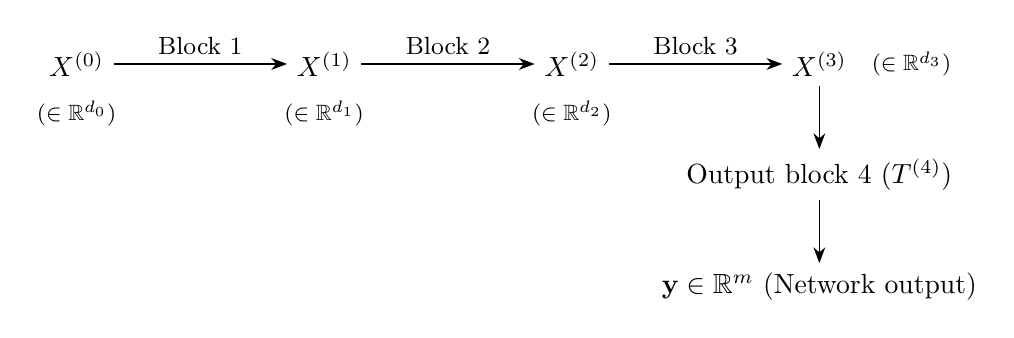
\begin{tikzpicture}[
    node distance=0.8cm and 2.2cm, % Vertical and horizontal node distances
    block/.style={font=\small}, % Style for block labels
    dim/.style={font=\footnotesize} % Style for dimension labels
  ]
    % Define nodes
    \node (X0)                                      {$X^{(0)}$};
    \node (L0) [below=0.07cm of X0, dim]             {$(\in \mathbb{R}^{d_0})$};
    \node (X1) [right=of X0]                        {$X^{(1)}$};
    \node (L1) [below=0.07cm of X1, dim]             {$(\in \mathbb{R}^{d_1})$};
    \node (X2) [right=of X1]                        {$X^{(2)}$};
    \node (L2) [below=0.07cm of X2, dim]             {$(\in \mathbb{R}^{d_2})$};
    \node (X3) [right=of X2]                        {$X^{(3)}$};
    \node (L3) [right=0.07cm of X3, dim]             {$(\in \mathbb{R}^{d_3})$};
    \node (OB) [below=of X3]                        {Output block 4 $(T^{(4)})$};
    \node (Y)  [below=of OB]                        {$\mathbf{y} \in \mathbb{R}^m$ (Network output)};

    % Draw arrows
    \draw[-{Stealth[length=2mm]}] (X0) -- node[above, block] {Block 1} (X1);
    \draw[-{Stealth[length=2mm]}] (X1) -- node[above, block] {Block 2} (X2);
    \draw[-{Stealth[length=2mm]}] (X2) -- node[above, block] {Block 3} (X3);
    \draw[-{Stealth[length=2mm]}] (X3) -- (OB); % Vertical arrow
    \draw[-{Stealth[length=2mm]}] (OB) -- (Y);  % Vertical arrow
\end{tikzpicture}
\end{center}
Here, $X^{(\ell)} = \mathbf{h}^{(\ell)}$ denotes the output vector of the $\ell$-th Sprecher block (we use both notations interchangeably for clarity in different contexts). Each block $T^{(\ell)}$ internally uses its own pair of shared splines $(\phi^{(\ell)}, \Phi^{(\ell)})$, mixing weights $\lambda^{(\ell)}$, shift $\eta^{(\ell)}$, and optionally lateral mixing parameters $(\tau^{(\ell)}, \omega^{(\ell)})$. The final output block $T^{(4)}$ maps the representation $X^{(3)}$ to the final $m$-dimensional output $\mathbf{y}$ without subsequent summation.

\subsection{Illustrative expansions (scalar output)}
To further clarify the compositional structure for the scalar output case ($m=1$), we write out the full expansions for networks with $L=1, 2, 3$ hidden layers.

\subsubsection{Single hidden layer ($L=1$)}\label{sec:single_layer}
For a network with architecture $d_{\mathrm{in}}\to[d_1]\to1$ (i.e., $d_0=d_{\mathrm{in}}$), the network computes:
$$f(\mathbf{x}) = \sum_{q=0}^{d_1-1} \mathbf{h}^{(1)}_q = \sum_{q=0}^{d_1-1} \Phi^{(1)}\Biggl(\sum_{i=1}^{d_0} \lambda^{(1)}_{i}\,\phi^{(1)}\Bigl(x_i+\eta^{(1)}\,q\Bigr)+\alpha q + \tau^{(1)} \sum_{j \in \mathcal{N}(q)} \omega_{q,j}^{(1)} s_j^{(1)}\Biggr).$$
When lateral mixing is disabled ($\tau^{(1)} = 0$ or $\mathcal{N}(q) = \emptyset$), this reduces to Sprecher's 1965 construction if we choose $d_1=2d_0+1$, identify $\phi^{(1)}=\phi$, $\Phi^{(1)}=\Phi$, $\lambda^{(1)}_{i} = \lambda_i$, and set $\alpha = 1$.

\subsubsection{Two hidden layers ($L=2$)}
Let the architecture be $d_0\to[d_1, d_2]\to1$. The intermediate output $\mathbf{h}^{(1)} \in \mathbb{R}^{d_1}$ is computed as:
$$\mathbf{h}^{(1)}_r=\Phi^{(1)}\Bigl(\sum_{i=1}^{d_0}\lambda^{(1)}_{i}\,\phi^{(1)}\Bigl(x_i+\eta^{(1)}\,r\Bigr)+\alpha r + \tau^{(1)} \sum_{j \in \mathcal{N}(r)} \omega_{r,j}^{(1)} s_j^{(1)}\Bigr),\quad r=0,\dots,d_1-1.$$
The second block computes $\mathbf{h}^{(2)} \in \mathbb{R}^{d_2}$ using $\mathbf{h}^{(1)}$ as input:
$$\mathbf{h}^{(2)}_q=\Phi^{(2)}\Bigl(\sum_{r=0}^{d_1-1}\lambda^{(2)}_{r}\,\phi^{(2)}\Bigl(\mathbf{h}^{(1)}_r+\eta^{(2)}\,q\Bigr)+\alpha q + \tau^{(2)} \sum_{j \in \mathcal{N}(q)} \omega_{q,j}^{(2)} s_j^{(2)}\Bigr),\quad q=0,\dots,d_2-1.$$
The final network output is the sum over the components of $\mathbf{h}^{(2)}$: $f(\mathbf{x})=\sum_{q=0}^{d_2-1}\mathbf{h}^{(2)}_q$. 

For the base architecture without optional enhancements, the fully expanded form reveals the nested compositional structure:
\begin{equation}\label{eq:two-layer-expanded}
f(\mathbf{x})=\sum_{q=0}^{d_2-1}\Phi^{(2)}\Biggl(\sum_{r=0}^{d_1-1}\lambda^{(2)}_{r}\,\phi^{(2)}\Biggl(\underbrace{\Phi^{(1)}\Biggl(\sum_{i=1}^{d_0}\lambda^{(1)}_{i}\,\phi^{(1)}\Bigl(x_i+\eta^{(1)}\,r\Bigr)+\alpha r\Biggr)}_{\text{Output of first block}}+\eta^{(2)}\,q\Biggr)+\alpha q\Biggr).
\end{equation}
This nested structure, where the output of $\Phi^{(1)}$ becomes the input to $\phi^{(2)}$, fundamentally departs from Sprecher's original construction and represents our empirically-motivated deep architecture.

\begin{remark}[Lateral mixing in expanded form]
When lateral mixing is enabled, the expanded forms become more complex. For instance, in the two-layer case, each $s_r^{(1)}$ term undergoes mixing before the $\Phi^{(1)}$ transformation, and similarly for $s_q^{(2)}$ before $\Phi^{(2)}$. We omit the full expansion for clarity, but note that lateral mixing represents an additional source of inter-dimensional coupling beyond the shifts, potentially enhancing the network's ability to capture correlations between output dimensions.
\end{remark}

\subsubsection{Three hidden layers ($L=3$)}
Let the architecture be $d_0\to [d_1, d_2, d_3]\to1$. The recursive definition involves:
$$\begin{aligned}
\mathbf{h}^{(1)}_r &= \Phi^{(1)}\Bigl(\sum_{i=1}^{d_0}\lambda^{(1)}_{i}\,\phi^{(1)}\Bigl(x_i+\eta^{(1)}\,r\Bigr)+\alpha r + \tau^{(1)} \sum_{j \in \mathcal{N}(r)} \omega_{r,j}^{(1)} s_j^{(1)}\Bigr),\quad r=0,\dots,d_1-1,\\[1mm]
\mathbf{h}^{(2)}_s &= \Phi^{(2)}\Bigl(\sum_{r=0}^{d_1-1}\lambda^{(2)}_{r}\,\phi^{(2)}\Bigl(\mathbf{h}^{(1)}_r+\eta^{(2)}\,s\Bigr)+\alpha s + \tau^{(2)} \sum_{j \in \mathcal{N}(s)} \omega_{s,j}^{(2)} s_j^{(2)}\Bigr),\quad s=0,\dots,d_2-1,\\[1mm]
\mathbf{h}^{(3)}_q &= \Phi^{(3)}\Bigl(\sum_{s=0}^{d_2-1}\lambda^{(3)}_{s}\,\phi^{(3)}\Bigl(\mathbf{h}^{(2)}_s+\eta^{(3)}\,q\Bigr)+\alpha q + \tau^{(3)} \sum_{j \in \mathcal{N}(q)} \omega_{q,j}^{(3)} s_j^{(3)}\Bigr),\quad q=0,\dots,d_3-1.
\end{aligned}$$
The network output is $f(\mathbf{x})=\sum_{q=0}^{d_3-1}\mathbf{h}^{(3)}_q$. 

\begin{remark}
These expansions highlight the compositional nature where the output of one Sprecher block, which is a vector of transformed values, serves as the input to the next. Each transformation layer involves its own pair of shared splines, learnable parameters, and optionally lateral mixing connections.
\end{remark}

\begin{remark}[Necessity of internal shifts]\label{rem:shiftneeded}
It is tempting to simplify the nested structures, for instance by removing the inner shift terms like $\eta^{(2)}q$ inside $\phi^{(2)}$. One might hypothesize that the outer splines $\Phi^{(\ell)}$ could absorb this shifting effect (yielding a single composite spline per Sprecher block). However, experiments (see Section \ref{sec:ablation_eta}) suggest that these internal shifts $\eta^{(\ell)}q$ applied to the inputs of the $\phi^{(\ell)}$ splines are crucial for the effective functioning of deeper Sprecher Networks. Removing them significantly degrades performance. The precise theoretical reason for their necessity in the multi-layer case, beyond their presence in Sprecher's original single-layer formula, warrants further investigation.
\end{remark}

\section{Comparison with related architectures}
To position Sprecher Networks accurately, we compare their core architectural features with Multi-Layer Perceptrons (MLPs), networks with learnable node activations (LANs/Adaptive-MLPs), and Kolmogorov-Arnold Networks (KANs).

\begin{table}[ht]
\centering
\caption{Architectural comparison of neural network families.}
\label{tab:arch_comparison}
\small % Use smaller font size if needed
\begin{tabular}{@{}lllll@{}}
\toprule
Feature                   & MLP                 & LAN / Adaptive-MLP & KAN                   & Sprecher Network (SN) \\ \midrule
\textbf{Learnable}        & Linear Weights      & Linear Weights     & Edge Splines          & Block Splines ($\phi, \Phi$) \\
\textbf{Components}       & (on edges)          & + Node Activations &                       & + Mixing Weights ($\lambda$) \\
                          &                     &                    &                       & + Shift Parameter ($\eta$) \\
                          &                     &                    &                       & + Lateral Mixing ($\tau, \omega$) \\
\textbf{Fixed components}   & Node Activations    & ---                & Node Summation        & Node Summation (implicit) \\
                          &                     &                    &                       & + Fixed Shifts ($+\alpha q$) \\
\textbf{Location of}      & Nodes               & Nodes              & Edges                 & Blocks \\
\textbf{Non-linearity}    & (Fixed)             & (Learnable)        & (Learnable)           & (Shared, Learnable) \\
\textbf{Node operation}     & Apply $\sigma(\cdot)$ & Apply $\sigma_{\text{learn}}(\cdot)$ & $\sum (\text{inputs})$ & Implicit in Block Formula \\
\textbf{Parameter sharing}  & None (typically)    & Activations? (Maybe) & None (typically)      & Splines ($\phi, \Phi$) per block \\
\textbf{Intra-layer mixing} & None & None & None & Lateral (cyclic/bidir.) \\
                           &      &      &      & $O(N)$ params \\
\textbf{Residual design}    & Matrix projection   & Matrix projection  & None (typically)      & Cyclic \\
                          & $O(N^2)$ per skip   & $O(N^2)$ per skip  &                       & $O(N)$ per skip \\
\textbf{Theoretical basis}  & UAT                 & UAT                & KAT (inspired)        & KAS (Sprecher, direct) \\
\textbf{Param scaling}    & $O(L N^2)$          & $O(L N^2 + L N G)$ & $O(L N^2 G)$          & $O(L N + L G)$ \\
                          &                     & (Approx.)          &                       & (Approx.) \\
\textbf{Memory complexity} & $O(L N^2)$          & $O(L N^2)$         & $O(L N^2 G)$          & $O(L N^2)$ parallel \\
                          &                     &                    &                       & $\mathbf{O(L N)}$ sequential \\
\bottomrule
\end{tabular}
\vspace{2mm}
\parbox{\textwidth}{\footnotesize \textit{Notes:} $L$=depth, $N$=average width, $G$=spline grid size/complexity. UAT=Universal Approx. Theorem, KAT=Kolmogorov-Arnold Theorem, KAS=Kolmogorov-Arnold-Sprecher. LAN details often follow KAN Appendix B \cite{liu2024kan}. Memory complexity includes both parameter storage and computation requirements, treating batch size as a constant. The ``sequential'' mode for SNs processes output dimensions iteratively rather than in parallel, maintaining mathematical equivalence while reducing memory usage. All architectures may optionally include normalization layers; SNs apply normalization to entire block outputs rather than individual activations.
\textit{The parameter scaling notation uses $N$ to denote a typical or average layer width for simplicity, following \cite{liu2024kan}. For architectures with varying widths $d_\ell$, the $LN^2$ terms should be understood as $\sum_{\ell} d_{\ell-1}d_{\ell}$ (MLP, LAN), the $LN^2G$ term for KAN as $(\sum_{\ell} d_{\ell-1}d_{\ell})G$, and the $LN$ term for SN as $\sum_{\ell} d_{\ell-1}$ (since SN uses weight vectors, not matrices), where the sum is over the relevant blocks/layers, for precise counts.}}
\end{table}

Table \ref{tab:arch_comparison} summarizes the key distinctions between these architectures. MLPs learn edge weights with fixed node activations, LANs add learnable node activations to this structure, KANs move learnability entirely to edge splines while eliminating linear weights, and SNs concentrate learnability in shared block-level splines, block-level shifts, mixing weights, and optionally lateral mixing connections. The critical difference for SNs is their use of weight vectors rather than matrices, which fundamentally reduces the dependence on width from quadratic to linear. This architectural choice can be understood through an analogy with convolutional neural networks: just as CNNs achieve parameter efficiency and improved generalization by sharing weights across spatial locations, SNs share weights across output dimensions within each block. In CNNs, spatial shifts provide the necessary diversity despite weight sharing; in SNs, the shifts $\eta q$ and the additive term $+\alpha q$, along with lateral mixing when enabled, play this diversifying role. This perspective reframes our architectural constraint not as a limitation, but as a principled form of weight sharing motivated by Sprecher's theorem, suggesting that SNs might be viewed as a ``convolutional'' approach to function approximation networks. While this weight sharing is theoretically justified for single-layer networks, its effectiveness in deep compositions remains an empirical finding that warrants further theoretical investigation. This combination of choices leads to SNs' distinctive parameter scaling of $O(L N + L G)$ compared to KANs' $O(L N^2 G)$ and unique memory complexity of $O(LN)$ in sequential mode.\footnote{The $O(LN)$ term includes contributions from mixing weights ($\lambda$), normalization parameters when used, lateral mixing parameters, and Cyclic residual connections. Each residual connection contributes at most $\max(d_{\mathrm{in}}, d_{\mathrm{out}})$ parameters, maintaining the linear scaling in width.}

Here, we provide a precise comparison between LANs and SNs. While the following proposition shows that SNs can be expressed as special cases of LANs with specific structural constraints, it is important to note that Sprecher's construction guarantees that this constrained form retains full expressivity in the single-layer case. This suggests that the extreme parameter sharing and structural constraints in SNs may serve as a beneficial inductive bias rather than a limitation.

\begin{definition}
A LAN is an MLP with learnable activation. More precisely, the model is defined as: 
$$
f(\mathbf{x}) = A^{(L)} \circ \sigma^{(L-1)} \circ A^{(L-1)} \circ \sigma^{(L-2)} \circ \cdots \circ \sigma^{(1)} \circ A^{(1)} (\mathbf{x}),
$$
where $A^{(k)} \colon \mathbb{R}^{d_{k-1}} \rightarrow \mathbb{R}^{d_k}$ is an affine map, and $\sigma^{(k)} \colon \mathbb{R} \rightarrow \mathbb{R}  $ is the activation function (applied coordinate-wise). In an MLP, the trainable parameters are the weights $W^{(k)}$ and biases $b^{(k)}$ of $A^{(k)}(\mathbf{x}) = W^{(k)}\mathbf{x} + b^{(k)}$ for $k = 1, \ldots, L$. In a LAN, $\sigma$ contains additional trainable parameters, e.g., the coefficients of a spline.
\end{definition}

\begin{remark}[Note on weight structure]
The following proposition uses matrix weights $\lambda_{i,q}^{(\ell)}$ to establish the connection between SNs and LANs. However, the architecture we propose and analyze throughout this paper uses vector weights $\lambda_i^{(\ell)}$ (following Sprecher's original formulation), where the same weights are shared across all output dimensions. This vector version represents an even more constrained special case of the LAN formulation shown below. The practical SN architecture with vector weights would require the weight matrices in the proposition to have repeated rows, i.e., $\lambda_{i,q}^{(\ell)} = \lambda_i^{(\ell)}$ for all $q$. This constraint is fundamental to maintaining the "true Sprecher" structure and achieving the characteristic $O(LN)$ parameter scaling. Additionally, when lateral mixing is enabled, the structure becomes more complex, requiring additional terms in the LAN representation to capture the intra-block communication.
\end{remark}

\begin{prop} \label{prop:SNareLAN}
    A matrix-weighted variant of a Sprecher Network (i.e., with per-output mixing weights $\lambda^{(\ell)}_{i,q}$ in each block) and with lateral mixing disabled is a LAN, where:
    \begin{itemize}
        \item in odd layers $k = 2\ell - 1$, the weight matrix $W^{(k)} \in \mathbb{R}^{d_\ell d_{\ell-1} \times d_{\ell-1}}$ is fixed to  $[I | \cdots | I]^\top$, where $I$ is the $d_{\ell-1} \times d_{\ell-1}$ identity matrix, the bias vector has only one learnable parameter $\eta^{(\ell)}$ and is structured as $b^{(k)} = \eta^{(\ell)}(0,\ldots,0, 1, \ldots, 1, \ldots, d_{\ell}-1, \ldots, d_{\ell}-1)^\top \in \mathbb{R}^{d_\ell d_{\ell-1}}$, and the activation is $\sigma^{(k)} = \phi^{(\ell)}$, 
        \item in even layers $k = 2\ell $, the learnable weight matrix $W^{(k)} \in \mathbb{R}^{d_\ell \times d_\ell d_{\ell-1}}$ is structured as
        \begin{align*}
            \begin{bmatrix}
                \lambda_{1,0}^{(\ell)} & \cdots & \lambda_{d_{\ell-1},0}^{(\ell)} & 0 &&& \cdots &&&0 \\
               0  &\cdots & 0 & \lambda_{1,1}^{(\ell)} & \cdots & \lambda_{d_{\ell-1},1}^{(\ell)} & 0 && \cdots & 0 \\
               &&&&&& \ddots \\
               0 &&&\cdots &&&0&\lambda_{1,d_\ell-1}^{(\ell)} & \cdots & \lambda_{d_{\ell-1},d_\ell-1}^{(\ell)}
            \end{bmatrix},
        \end{align*} 
        the bias is fixed to $b^{(k)} = \alpha(0,\ldots, d_\ell-1)^\top \in \mathbb{R}^{d_\ell}$, and the activation is $\sigma^{(k)} = \Phi^{(\ell)}$. 
    \end{itemize}
\end{prop}
\begin{proof}
    Follows immediately by inspecting \eqref{eq:SN} with $\tau^{(\ell)} = 0$ (no lateral mixing).
\end{proof}

\begin{remark}[Understanding the LAN representation]
The representation of SNs as LANs in Proposition~\ref{prop:SNareLAN} uses an expanded 
intermediate state space. Each Sprecher block is decomposed into two LAN layers:
\begin{itemize}
\item The first layer expands the input $\mathbf{h}^{(\ell-1)} \in \mathbb{R}^{d_{\ell-1}}$ 
to $\mathbb{R}^{d_\ell d_{\ell-1}}$ by creating $d_\ell$ shifted copies, where the 
$(q \cdot d_{\ell-1} + i)$-th component contains $\phi^{(\ell)}(h^{(\ell-1)}_i + \eta^{(\ell)} q)$.
\item The second layer applies the mixing weights $\lambda^{(\ell)}_{i,q}$ to select and sum 
the appropriate components for each output $q$, adds the shift $\alpha q$, and applies $\Phi^{(\ell)}$.
\end{itemize}
This construction shows that while SNs can be expressed within the LAN framework, they 
represent a highly structured special case with specific weight patterns and an expanded 
intermediate dimension of $O(d_{\ell-1} d_\ell)$ between each pair of SN layers. The inclusion of lateral mixing would further complicate this representation, requiring additional structure to capture the intra-block communication.
\end{remark}

While this proposition shows that SNs are special cases of LANs with specific structural constraints, Sprecher's construction guarantees that this constrained form retains full expressivity. In Sprecher's original construction, $\eta$ can be chosen as a universal constant rather than a learnable parameter. This, combined with Proposition \ref{prop:SNareLAN}, implies that LANs do not lose expressivity when constraining biases to specific structured forms.

\begin{figure}[h!]
    \centering  
\begin{tikzcd}[ampersand replacement=\&]
    \& \textnormal{LAN} \\
    \textnormal{MLP} \&\& \textnormal{SN}
    \arrow[hook, from=2-1, to=1-2]
    \arrow[hook', from=2-3, to=1-2]
\end{tikzcd}
    \caption{Diagram illustrating the dependencies between the models, in terms of learnable parameters. MLPs are LANs with fixed activation function, while SNs are LANs with a particular parameter structure (Proposition \ref{prop:SNareLAN}).}
    \label{fig:model_dependencies}
\end{figure}

\begin{remark}[Domain considerations]
The above proposition assumes that the spline functions $\phi^{(\ell)}$ can handle inputs outside their original domain $[0,1]$, which may arise due to the shifts $\eta^{(\ell)}q$. While Sprecher's theoretical construction extends $\phi$ appropriately, practical implementations typically compute exact theoretical bounds for all spline domains based on the network structure, ensuring that all evaluations fall within the spline's operating range through dynamic domain updates.
\end{remark}

\section{Parameter counting and efficiency as a trade-off}
A key consequence of adhering to the vector-based weighting scheme inspired by Sprecher's formula is a dramatic reduction in parameters compared to standard architectures. This represents a strong architectural constraint that may serve as either a beneficial inductive bias or a limitation, depending on the target function class. The specific design of SNs, particularly the sharing of splines and use of weight vectors rather than matrices, leads to a distinctive parameter scaling that warrants careful analysis.

Let's assume a network of depth $L$ (meaning $L$ hidden layers, thus $L$ blocks for scalar output or $L+1$ for vector output), with an average layer width $N$. We denote the input dimension as $N_{in}$ when it differs significantly from the hidden layer widths. Let $G$ be the number of intervals used for the piecewise-linear splines (implying $G+1$ knots). For simplicity, we approximate the number of parameters per spline as $O(G)$.

The parameter counts for different architectures scale as follows. MLPs primarily consist of linear weight matrices, leading to a total parameter count dominated by these weights, scaling as $O(L N^2)$. LANs (Adaptive-MLPs) have both linear weights ($O(L N^2)$) and learnable activations; if each of the $N$ nodes per layer has a learnable spline, this adds $O(L N G)$ parameters, for a total of $O(L N^2 + L N G)$. KANs replace linear weights with learnable edge splines, with $O(N^2)$ edges between layers. If each edge has a spline with $O(G)$ parameters, the total count per layer is $O(N^2 G)$, leading to an overall scaling of $O(L N^2 G)$.

Sprecher Networks have a fundamentally different structure. Each block $\ell$ contains mixing weights $\lambda^{(\ell)}$ with $O(d_{\ell-1})$ parameters, where $d_{\ell-1}$ is the input dimension to that block (crucially, these are vectors, not matrices), shared splines $\phi^{(\ell)}, \Phi^{(\ell)}$ with $2 \times O(G) = O(G)$ parameters per block independent of $N$, and a shift parameter $\eta^{(\ell)}$ with $O(1)$ parameter per block. When lateral mixing is enabled, each block additionally contains a lateral scale parameter $\tau^{(\ell)}$ with $O(1)$ parameter and mixing weights $\omega^{(\ell)}$ with $O(d_\ell)$ parameters (specifically $d_\ell$ for cyclic, $2d_\ell$ for bidirectional). When normalization is used, each block may have an associated normalization layer adding $O(N)$ parameters (specifically $2N$ for the affine transformation). When residual connections are used, they add at most $O(N)$ parameters per block using the Cyclic approach (specifically $\max(d_{\ell-1}, d_\ell)$ for block $\ell$, or just 1 when dimensions match). Summing over $L$ (or $L+1$) blocks, the total parameter count scales approximately as $O(LN + LG + L)$, where the linear dependence on $N$ now includes mixing weights, optional normalization parameters, lateral mixing weights, and residual connections.

Beyond parameter efficiency, SNs also admit memory-efficient computation strategies. While standard implementations require $O(B \cdot d_{\mathrm{in}} \cdot d_{\mathrm{out}})$ memory per block for batch size $B$, a sequential evaluation strategy reduces this to $O(B \cdot \max(d_{\mathrm{in}}, d_{\mathrm{out}}))$. Combined with the $O(LN)$ parameter scaling, this makes SNs particularly suitable for exploring wide architectures that would be infeasible with conventional networks due to memory constraints rather than parameter counts. For instance, a single block with architecture $512 \to [512] \to 1$ requires only a few thousand parameters but can exhaust memory in standard parallel computation; the sequential approach makes such architectures trainable with modest memory overhead. The total memory complexity for SNs thus becomes $O(LN)$ when treating batch size as a constant, compared to MLPs' $O(LN^2)$ total memory requirement.

This scaling reveals the crucial trade-off: SNs achieve a reduction from $O(LN^2)$ to $O(LN)$ in both parameter count and memory complexity by using weight vectors rather than matrices. Additionally, in KANs, the spline complexity $G$ multiplies the $N^2$ term ($O(L N^2 G)$), while in SNs, due to spline sharing within blocks, it appears as an additive term ($O(L G)$). This suggests potential for significant parameter and memory savings, particularly when high spline resolution ($G$) is required for accuracy or when the layer width ($N$) is moderate to large.

This extreme parameter sharing represents a fundamental architectural bet: that the structure imposed by Sprecher's theorem, using only weight vectors with output diversity through shifts and lateral mixing, provides a beneficial inductive bias that outweighs the reduction in parameter flexibility. The empirical observation that training remains feasible (albeit sometimes requiring more iterations) with vector weights suggests this bet may be justified for certain function classes. Moreover, viewing this constraint through the lens of weight sharing in CNNs provides a new perspective: both architectures sacrifice parameter flexibility for a structured representation that has proven effective in practice, though for SNs the theoretical justification comes from Sprecher's theorem rather than domain-specific intuitions about spatial invariance. The addition of lateral mixing provides a middle ground, allowing some cross-dimensional communication while maintaining the overall parameter efficiency. Whether this constraint serves as beneficial regularization or harmful limitation likely depends on the specific problem domain and the alignment between the target function's structure and the inductive bias imposed by the SN architecture.

\subsection{Illustrative parameter comparisons (hypothetical examples)}
We present parameter count comparisons based on architectures reported in \cite{liu2024kan} to illustrate the potential parameter efficiency of SNs. Note that these examples are hypothetical; while the KAN architectures are from their paper, the SN results are theoretical projections that require empirical validation. Optimal architectures for SNs may differ from those of KANs due to the shared spline structure.

\paragraph{PDE solving example (KAN Ref § 3.4):}
KAN architecture $[2, 10, 1]$, reported effective. $N_{in}=2, N_{hid}=10, N_{out}=1$.
\begin{itemize}
    \item \textbf{KAN (est.):} $(2\times10 + 10\times1) = 30$ edges/splines. KANs use B-splines with $G=20$ intervals, $k=3$ ($G+k \approx 23$ params/spline). Total KAN params $\approx 30 \times 23 = 690$.
    \item \textbf{SN (hypothetical):} Architecture $2 \to [10] \to 1$. $L=1$ hidden layer, scalar output means $L=1$ block total. SNs use piecewise linear splines with $G=20$ intervals ($G+1 = 21$ params/spline). Shared splines: $2 \times 21 = 42$. Mixing weights: $d_0 = 2$ (vector weights). Shift $\eta^{(1)}$: $1$. If lateral mixing enabled (cyclic): $\tau^{(1)}$: $1$, $\omega^{(1)}$: $10$. Total SN params $\approx 42 + 2 + 1 + 1 + 10 = 56$ (with lateral mixing) or $45$ (without).
    \item \textbf{Potential advantage:} For equivalent structure, theoretical reduction factor $\approx 12-15$x. Actual performance requires empirical validation.
\end{itemize}

\paragraph{Knot theory example (KAN Ref § 4.3):}
Pruned KAN $[17, 1, 14]$, with B-splines using $G=3$ intervals, $k=3$ ($G+k \approx 6$ params/spline).
\begin{itemize}
    \item \textbf{KAN (est.):} $(17\times1 + 1\times14) = 31$ edges/splines. Total KAN params $\approx 31 \times 6 = 186$.
    \item \textbf{SN (hypothetical):} Architecture $17 \to [1] \to 14$. $L=1$ hidden layer, vector output means $L+1=2$ blocks total. Using piecewise linear splines with $G=3$ intervals: $2(L+1) \times (G+1) = 4 \times 4 = 16$. Mixing weights: $d_0 + d_1 = 17 + 1 = 18$ (vector weights). Shifts $\eta^{(1)}, \eta^{(2)}$: $2$. If lateral mixing enabled (cyclic) for both blocks: $\tau^{(1)}, \tau^{(2)}$: $2$, $\omega^{(1)}$: $1$, $\omega^{(2)}$: $14$. Total SN params $\approx 16 + 18 + 2 + 2 + 1 + 14 = 53$ (with lateral mixing) or $36$ (without).
    \item \textbf{Potential advantage:} Theoretical reduction factor $\approx 3.5-5$x. The narrow intermediate dimension $d_1=1$ might pose challenges for SN training.
\end{itemize}

These calculations illustrate the dramatic parameter reduction possible with SNs, but they also highlight a crucial practical consideration: the optimal architecture for SNs likely differs substantially from that of MLPs or KANs. With vector weights providing only linear scaling in width, SNs may require wider or deeper architectures to achieve comparable expressivity. The art of architecture selection for SNs involves balancing the parameter efficiency against the need for sufficient expressivity: a trade-off that remains poorly understood and likely depends strongly on the problem domain. Early empirical evidence suggests that SNs excel when the target function aligns well with their compositional, shift-based structure, but may require more iterations when forced to approximate functions that require truly independent processing of different output dimensions. The addition of lateral mixing partially addresses this limitation by enabling limited cross-dimensional communication.

\section{Theoretical aspects and open questions}\label{sec:universality}

\subsection{Relation to Sprecher (1965) and universality}
As shown in Section \ref{sec:single_layer}, a single-layer ($L=1$) Sprecher Network (SN) reduces exactly to Sprecher's constructive representation \eqref{eq:sprecher_original} when lateral mixing and residuals are disabled (i.e., $\tau=0$ and no residual connection), with the additive shift implemented by $\alpha q$ (set $\alpha=1$ to match \eqref{eq:sprecher_original}). In his 1965 paper, Sprecher proved that for any continuous function $f:[0,1]^n\to\mathbb{R}$ there exist a \emph{single} nondecreasing univariate function $\phi$, a continuous univariate function $\Phi$, real constants $\lambda_1,\ldots,\lambda_n$ and $\eta$, and an integer upper index $2n$ such that the representation \eqref{eq:sprecher_original} holds \cite{sprecher1965}. This immediately implies:

\begin{theorem}[Universality of single-layer SNs]\label{thm:ua_single_layer}
For any $n\ge 1$ and any $f\in C([0,1]^n)$, there exists a single-layer SN with $\tau=0$ and no residual connection that represents $f$ exactly in the form \eqref{eq:sprecher_original} (taking $d_{\mathrm{out}}=2n+1$ and $\alpha=1$). In particular, for every $\epsilon>0$ there is a single-layer SN (with $\tau=0$ and no residual) such that $\sup_{\mathbf{x}\in[0,1]^n}|f(\mathbf{x})-\hat f(\mathbf{x})|<\epsilon$.
\end{theorem}

Thus, single-layer SNs inherit (indeed, contain) the family given by Sprecher's representation. In practice, however, we do not fit arbitrary $C^2$ univariate functions $\phi$ and $\Phi$ exactly; we parameterize them as splines. This motivates the following finite-parameter approximation analysis, which also clarifies how optional \emph{lateral mixing} (controlled by $\tau$ and $\omega$) and cyclic residuals affect constants but not rates.

\medskip
\noindent\textbf{Notation for a single block.}
A (possibly mixed) Sprecher block $T:\mathbb{R}^{d_{\mathrm{in}}}\to\mathbb{R}^{d_{\mathrm{out}}}$ acts componentwise as
\[
[T(\mathbf{z})]_q \;=\; \Phi\!\Biggl(\,\underbrace{\sum_{i=1}^{d_{\mathrm{in}}}\lambda_i\,\phi(z_i+\eta q)+\alpha q}_{=:s_q}\;+\;\tau\sum_{j\in\mathcal{N}(q)}\omega_{qj}\,s_j\Biggr),
\quad q=0,\ldots,d_{\mathrm{out}}-1,
\]
where $\lambda\in\mathbb{R}^{d_{\mathrm{in}}}$, $\eta,\alpha,\tau\in\mathbb{R}$, $\mathcal{N}(q)$ specifies the (optional) neighborhood used for lateral mixing, and $\omega=(\omega_{qj})$ are the mixing weights. When a cyclic residual connection is present, the block output is $T_{\mathrm{res}}(\mathbf{z})=T(\mathbf{z})+R(\mathbf{z})$; the analysis below applies to $T$ and extends to $T_{\mathrm{res}}$ by adding the Lipschitz constant of $R$ where relevant.

\begin{lemma}[Single block approximation with piecewise-linear splines]\label{lem:single_block}
Fix $B_{\mathrm{in}}>0$ and assume $\mathbf{z}\in\mathcal{B}_{\mathrm{in}}:=[-B_{\mathrm{in}},B_{\mathrm{in}}]^{d_{\mathrm{in}}}$. Let
\[
I_\phi := \bigl[-B_{\mathrm{in}}-|\eta|(d_{\mathrm{out}}-1),\; B_{\mathrm{in}}+|\eta|(d_{\mathrm{out}}-1)\bigr],
\quad
M_\phi := \|\phi\|_{L^\infty(I_\phi)}.
\]
Define
\[
B_\omega:=\sup_{q}\sum_{j\in\mathcal{N}(q)}|\omega_{qj}|,
\qquad
R_{\mathrm{mix}}:=1+|\tau|\,B_\omega,
\qquad
M_s := \|\lambda\|_{1}\,M_\phi + |\alpha|\,(d_{\mathrm{out}}-1),
\]
and set $I_\Phi := [-R_{\mathrm{mix}}M_s,\; R_{\mathrm{mix}}M_s]$. Assume $\phi,\Phi\in C^2$ on neighborhoods of $I_\phi$ and $I_\Phi$, respectively. Let $\hat\phi$ and $\hat\Phi$ be the (shape-preserving) piecewise-linear interpolants of $\phi$ on a uniform grid of $G_\phi\ge 2$ knots over $I_\phi$ and of $\Phi$ on a uniform grid of $G_\Phi\ge 2$ knots over $I_\Phi$; write
\[
h_\phi:=\frac{|I_\phi|}{G_\phi-1},\quad h_\Phi:=\frac{|I_\Phi|}{G_\Phi-1},\quad
M_{\phi''}:=\|\phi''\|_{L^\infty(I_\phi)},\quad M_{\Phi''}:=\|\Phi''\|_{L^\infty(I_\Phi)}.
\]
Define $\hat T$ by replacing $(\phi,\Phi)$ with $(\hat\phi,\hat\Phi)$ in $T$ (keeping the same $\lambda,\eta,\alpha,\tau,\omega,\mathcal{N}$). Then, for all $\mathbf{z}\in\mathcal{B}_{\mathrm{in}}$,
\begin{equation}\label{eq:single_block_sup}
\|T(\mathbf{z})-\hat T(\mathbf{z})\|_\infty
\;\le\;
L_\Phi\,R_{\mathrm{mix}}\,\|\lambda\|_{1}\,\delta_\phi\;+\;\delta_\Phi,
\qquad
\delta_\phi:=\frac{M_{\phi''}}{8}h_\phi^2,\ \ \delta_\Phi:=\frac{M_{\Phi''}}{8}h_\Phi^2,
\end{equation}
where $L_\Phi:=\|\Phi'\|_{L^\infty(I_\Phi)}$. Equivalently,
\[
\|T(\mathbf{z})-\hat T(\mathbf{z})\|_\infty
\;\le\;
K_T\cdot \max\{h_\phi^2,h_\Phi^2\}
\quad\text{with}\quad
K_T:=\frac{1}{8}\Bigl(L_\Phi\,R_{\mathrm{mix}}\,\|\lambda\|_{1}\,M_{\phi''}+M_{\Phi''}\Bigr).
\]
The same bounds hold for a block with a (shared) cyclic residual $T_{\mathrm{res}}=T+R$, since $R$ cancels when $T$ and $\hat T$ share the same residual path.
\end{lemma}

\begin{proof}
On each subinterval of the uniform grid for $I_\phi$ (resp.\ $I_\Phi$) of length $h_\phi$ (resp.\ $h_\Phi$), the classical bound for piecewise-linear interpolation of a $C^2$ function gives
\[
\|\phi-\hat\phi\|_{L^\infty(I_\phi)}\le \frac{M_{\phi''}}{8}h_\phi^2=:\delta_\phi,
\qquad
\|\Phi-\hat\Phi\|_{L^\infty(I_\Phi)}\le \frac{M_{\Phi''}}{8}h_\Phi^2=:\delta_\Phi.
\]
For fixed $\mathbf{z}$ and $q$, write $s_q=\sum_i\lambda_i\,\phi(z_i+\eta q)+\alpha q$ and $\hat s_q$ the analogous quantity with $\hat\phi$. Then
\[
|s_q-\hat s_q|\;\le\;\sum_{i=1}^{d_{\mathrm{in}}}|\lambda_i|\,\|\phi-\hat\phi\|_{L^\infty(I_\phi)}
\;\le\;\|\lambda\|_{1}\,\delta_\phi.
\]
Define the pre-mixing scalars $\tilde s_q:=s_q+\tau\sum_{j\in\mathcal{N}(q)}\omega_{qj}s_j$ and $\hat{\tilde s}_q:=\hat s_q+\tau\sum_{j\in\mathcal{N}(q)}\omega_{qj}\hat s_j$. Using the triangle inequality and the definition of $B_\omega$,
\[
|\tilde s_q-\hat{\tilde s}_q|
\;\le\;
|s_q-\hat s_q| + |\tau| \sum_{j\in\mathcal{N}(q)}|\omega_{qj}|\,|s_j-\hat s_j|
\;\le\; R_{\mathrm{mix}}\cdot \sup_{j}|s_j-\hat s_j|
\;\le\; R_{\mathrm{mix}}\,\|\lambda\|_{1}\,\delta_\phi.
\]
Next, since a linear interpolant lies in the convex hull of the function values at the grid endpoints, we have
\[
\|\hat\phi\|_{L^\infty(I_\phi)} \;\le\; \|\phi\|_{L^\infty(I_\phi)}=M_\phi.
\]
Hence $|s_j|\le M_s$ and $|\hat s_j|\le M_s$, which implies $|\tilde s_q|\le R_{\mathrm{mix}}M_s$ and $|\hat{\tilde s}_q|\le R_{\mathrm{mix}}M_s$. Therefore $\tilde s_q,\hat{\tilde s}_q\in I_\Phi$, and
\[
|T(\mathbf{z})_q-\hat T(\mathbf{z})_q|
=\bigl|\Phi(\tilde s_q)-\hat\Phi(\hat{\tilde s}_q)\bigr|
\le \underbrace{|\Phi(\tilde s_q)-\Phi(\hat{\tilde s}_q)|}_{\le L_\Phi |\tilde s_q-\hat{\tilde s}_q|}
+ \underbrace{|\Phi(\hat{\tilde s}_q)-\hat\Phi(\hat{\tilde s}_q)|}_{\le \delta_\Phi}.
\]
Combining the bounds and taking the maximum over $q$ yields \eqref{eq:single_block_sup}. If a residual path $R$ is present and shared between $T$ and $\hat T$, then $T_{\mathrm{res}}-\hat T_{\mathrm{res}}=(T-\hat T)+(R-R)=(T-\hat T)$, so the same inequalities apply.
\end{proof}

\begin{lemma}[Lipschitz constant of a Sprecher block]\label{lem:block_lip}
Assume $\phi$ and $\Phi$ are Lipschitz on $I_\phi$ and $I_\Phi$ with constants $L_\phi:=\|\phi'\|_{L^\infty(I_\phi)}$ and $L_\Phi:=\|\Phi'\|_{L^\infty(I_\Phi)}$, respectively. Then $T$ is $L_T$-Lipschitz on $\mathcal{B}_{\mathrm{in}}$ in the $\ell_\infty$ norm with
\[
L_T \;\le\; L_\Phi\,R_{\mathrm{mix}}\,\|\lambda\|_1\,L_\phi,
\]
where $R_{\mathrm{mix}}=1+|\tau|\,B_\omega$ as in Lemma~\ref{lem:single_block}. If a residual path $R$ (shared between the exact and approximated networks) is present with Lipschitz constant $L_R$ on $\mathcal{B}_{\mathrm{in}}$, then $T_{\mathrm{res}}=T+R$ is $(L_T+L_R)$-Lipschitz.
\end{lemma}

\begin{proof}
For $\mathbf{z},\mathbf{z}'\in\mathcal{B}_{\mathrm{in}}$ and each $q$,
\[
\bigl|s_q(\mathbf{z})-s_q(\mathbf{z}')\bigr|
\le \sum_i |\lambda_i|\,\bigl|\phi(z_i+\eta q)-\phi(z_i'+\eta q)\bigr|
\le \|\lambda\|_1\,L_\phi\,\|\mathbf{z}-\mathbf{z}'\|_\infty.
\]
Therefore,
\[
\bigl|\tilde s_q(\mathbf{z})-\tilde s_q(\mathbf{z}')\bigr|
\le \Bigl(1+|\tau|\,\sum_{j\in\mathcal{N}(q)}|\omega_{qj}|\Bigr)\,\|\lambda\|_1\,L_\phi\,\|\mathbf{z}-\mathbf{z}'\|_\infty
\le R_{\mathrm{mix}}\|\lambda\|_1 L_\phi\,\|\mathbf{z}-\mathbf{z}'\|_\infty,
\]
and hence
\[
|T(\mathbf{z})_q-T(\mathbf{z}')_q|
\le L_\Phi\,|\tilde s_q(\mathbf{z})-\tilde s_q(\mathbf{z}')|
\le L_\Phi R_{\mathrm{mix}}\|\lambda\|_1 L_\phi\,\|\mathbf{z}-\mathbf{z}'\|_\infty.
\]
Taking the maximum over $q$ gives the claimed bound for $T$, and adding $L_R$ handles $T_{\mathrm{res}}$ by the triangle inequality.
\end{proof}

\begin{lemma}[Error composition]\label{lem:error_composition}
Consider an $L$-block SN (with optional lateral mixing and cyclic residuals at each block). Let $T^{(\ell)}:\mathbb{R}^{d_{\ell-1}}\to\mathbb{R}^{d_{\ell}}$ denote the $\ell$-th block map on the exact network and $\hat T^{(\ell)}$ its spline-approximated counterpart (same $\lambda,\eta,\alpha,\tau,\omega$ but $(\phi,\Phi)$ replaced by $(\hat\phi,\hat\Phi)$). Assume there exist bounded sets $\mathcal{B}_{\ell}\subset\mathbb{R}^{d_{\ell}}$ such that for all inputs $\mathbf{x}\in[0,1]^n$,
\[
\mathbf{h}^{(\ell)}(\mathbf{x}) := T^{(\ell)}\!\circ\cdots\circ T^{(1)}(\mathbf{x}) \in \mathcal{B}_{\ell}
\quad\text{and}\quad
\hat{\mathbf{h}}^{(\ell)}(\mathbf{x}) := \hat T^{(\ell)}\!\circ\cdots\circ \hat T^{(1)}(\mathbf{x}) \in \mathcal{B}_{\ell},
\]
and suppose each $T^{(\ell)}$ is $L_{T^{(\ell)}}$-Lipschitz on $\mathcal{B}_{\ell-1}$. If $\varepsilon_\ell:=\sup_{\mathbf{z}\in\mathcal{B}_{\ell-1}}\|T^{(\ell)}(\mathbf{z})-\hat T^{(\ell)}(\mathbf{z})\|_\infty$, then for $E_\ell:=\sup_{\mathbf{x}\in[0,1]^n}\|\mathbf{h}^{(\ell)}(\mathbf{x})-\hat{\mathbf{h}}^{(\ell)}(\mathbf{x})\|_\infty$ we have
\begin{equation}\label{eq:error_composition_result}
E_\ell \;\le\; \sum_{j=1}^{\ell}\left(\prod_{m=j+1}^{\ell} L_{T^{(m)}}\right)\varepsilon_j,
\end{equation}
with the empty product equal to $1$.
\end{lemma}

\begin{proof}
The case $\ell=1$ is $E_1\le \varepsilon_1$. Assume the claim for $\ell-1$. Then, for any $\mathbf{x}$,
\begin{align*}
\|\mathbf{h}^{(\ell)}(\mathbf{x})-\hat{\mathbf{h}}^{(\ell)}(\mathbf{x})\|_\infty
&= \|T^{(\ell)}(\mathbf{h}^{(\ell-1)}(\mathbf{x})) - \hat T^{(\ell)}(\hat{\mathbf{h}}^{(\ell-1)}(\mathbf{x}))\|_\infty\\
&\le \underbrace{\|T^{(\ell)}(\mathbf{h}^{(\ell-1)}(\mathbf{x})) - T^{(\ell)}(\hat{\mathbf{h}}^{(\ell-1)}(\mathbf{x}))\|_\infty}_{\le L_{T^{(\ell)}}\,\|\mathbf{h}^{(\ell-1)}(\mathbf{x})-\hat{\mathbf{h}}^{(\ell-1)}(\mathbf{x})\|_\infty}
+ \underbrace{\|T^{(\ell)}-\hat T^{(\ell)}\|_{\infty,\mathcal{B}_{\ell-1}}}_{\le \varepsilon_\ell}\\
&\le L_{T^{(\ell)}} E_{\ell-1} + \varepsilon_\ell,
\end{align*}
and the induction hypothesis gives \eqref{eq:error_composition_result}.
\end{proof}

\begin{corollary}[Global spline approximation rate for SNs with piecewise-linear splines]\label{cor:sprecher_rate}
Let $f:[0,1]^n\to\mathbb{R}$ be realized by an ideal $L$-block SN (possibly with lateral mixing and cyclic residuals) with scalar output. For each block $\ell=1,\dots,L$, let $B_{\mathrm{in}}^{(\ell)}:=\sup\{\|\mathbf{z}\|_\infty:\mathbf{z}\in\mathcal{B}_{\ell-1}\}$. Assume:
\begin{enumerate}[label=\textup{(\roman*)}]
\item $\phi^{(\ell)},\Phi^{(\ell)}\in C^2$ on neighborhoods of the intervals
\[
I_\phi^{(\ell)} := \bigl[-B_{\mathrm{in}}^{(\ell)}-|\eta^{(\ell)}|(d_{\ell}-1),\; B_{\mathrm{in}}^{(\ell)}+|\eta^{(\ell)}|(d_{\ell}-1)\bigr],
\quad
I_\Phi^{(\ell)} := \bigl[-R_{\mathrm{mix}}^{(\ell)}M_s^{(\ell)},\; R_{\mathrm{mix}}^{(\ell)}M_s^{(\ell)}\bigr],
\]
with $M_s^{(\ell)}:=\|\lambda^{(\ell)}\|_{1}\|\phi^{(\ell)}\|_{L^\infty(I_\phi^{(\ell)})}+|\alpha^{(\ell)}|(d_\ell-1)$ and $R_{\mathrm{mix}}^{(\ell)}:=1+|\tau^{(\ell)}|\,B_\omega^{(\ell)}$, $B_\omega^{(\ell)}:=\sup_q\sum_{j\in\mathcal{N}^{(\ell)}(q)}|\omega^{(\ell)}_{qj}|$;
\item the structural parameters are bounded: $\|\lambda^{(\ell)}\|_{1}\le \Lambda_1$, $|\eta^{(\ell)}|\le H$, $|\alpha^{(\ell)}|\le A$, $|\tau^{(\ell)}|\le T$, and $B_\omega^{(\ell)}\le \Omega$;
\item there exist bounded sets $\mathcal{B}_\ell$ such that the exact and approximated forward passes both remain in $\mathcal{B}_\ell$ for all inputs in $[0,1]^n$ (bounded propagation).
\end{enumerate}
Construct $\hat\phi^{(\ell)}$ and $\hat\Phi^{(\ell)}$ as the piecewise-linear interpolants on uniform grids with $G_\phi^{(\ell)}\ge2$ and $G_\Phi^{(\ell)}\ge2$ knots on $I_\phi^{(\ell)}$ and $I_\Phi^{(\ell)}$, respectively, and write $h_\phi^{(\ell)}:=|I_\phi^{(\ell)}|/(G_\phi^{(\ell)}-1)$ and $h_\Phi^{(\ell)}:=|I_\Phi^{(\ell)}|/(G_\Phi^{(\ell)}-1)$. Then, with
\[
\delta_\phi^{(\ell)}:=\frac{\|\phi^{(\ell)''}\|_{L^\infty(I_\phi^{(\ell)})}}{8}\,\bigl(h_\phi^{(\ell)}\bigr)^2, \qquad
\delta_\Phi^{(\ell)}:=\frac{\|\Phi^{(\ell)''}\|_{L^\infty(I_\Phi^{(\ell)})}}{8}\,\bigl(h_\Phi^{(\ell)}\bigr)^2,
\]
the blockwise error satisfies
\[
\varepsilon_\ell
:=\sup_{\mathbf{z}\in\mathcal{B}_{\ell-1}}\|T^{(\ell)}(\mathbf{z})-\hat T^{(\ell)}(\mathbf{z})\|_\infty
\ \le\ L_{\Phi}^{(\ell)}\,R_{\mathrm{mix}}^{(\ell)}\,\|\lambda^{(\ell)}\|_{1}\,\delta_\phi^{(\ell)}\;+\;\delta_\Phi^{(\ell)},
\]
where $L_{\Phi}^{(\ell)}:=\|\Phi^{(\ell)'}\|_{L^\infty(I_\Phi^{(\ell)})}$. Consequently, by Lemma~\ref{lem:error_composition},
\[
\sup_{\mathbf{x}\in[0,1]^n}|f(\mathbf{x})-\hat f(\mathbf{x})|
\;\le\;
\sum_{j=1}^{L}\left(\prod_{m=j+1}^{L}L_{T^{(m)}}\right)\Bigl(L_{\Phi}^{(j)}\,R_{\mathrm{mix}}^{(j)}\,\|\lambda^{(j)}\|_{1}\,\delta_\phi^{(j)}+\delta_\Phi^{(j)}\Bigr),
\]
with $L_{T^{(m)}}$ any Lipschitz constant of the $m$-th block on $\mathcal{B}_{m-1}$ (e.g.\ from Lemma~\ref{lem:block_lip}, plus the residual-path constant when present). In particular, if $G_\phi^{(\ell)}=G_\Phi^{(\ell)}=G$ for all $\ell$, then with $h:=\max_\ell\{|I_\phi^{(\ell)}|,|I_\Phi^{(\ell)}|\}/(G-1)$ we obtain
\[
\sup_{\mathbf{x}\in[0,1]^n}|f(\mathbf{x})-\hat f(\mathbf{x})|
\;=\; \mathcal{O}\!\left(h^2\right)
\;=\; \mathcal{O}\!\left(G^{-2}\right),
\]
with constants depending on $\{\|\lambda^{(\ell)}\|_{1},L_{\phi^{(\ell)}},L_{\Phi}^{(\ell)},R_{\mathrm{mix}}^{(\ell)},\|\phi^{(\ell)''}\|_\infty,\|\Phi^{(\ell)''}\|_\infty,L_{T^{(\ell)}}\}_{\ell=1}^L$ and on the bounded-propagation sets $\{\mathcal{B}_\ell\}$.
\end{corollary}

\begin{remark}[Impact of lateral mixing and cyclic residuals]
Lateral mixing appears only inside the argument of $\Phi$ and inflates constants via $R_{\mathrm{mix}}^{(\ell)}=1+|\tau^{(\ell)}|\,B_\omega^{(\ell)}$ (with $B_\omega^{(\ell)}\le \|\omega^{(\ell)}\|_\infty N_{\max}^{(\ell)}$); it does not change the $G^{-2}$ rate. If a cyclic residual path $R$ is present and shared between $T^{(\ell)}$ and $\hat T^{(\ell)}$, it cancels in the blockwise difference and thus does not affect $\varepsilon_\ell$, but it \emph{does} contribute additively to $L_{T^{(\ell)}}$ in \eqref{eq:error_composition_result}. For example, when $d_{\mathrm{in}}=d_{\mathrm{out}}$ and $R(\mathbf{z})=w_{\mathrm{res}}\mathbf{z}$, we may take $L_{T^{(\ell)}}\le L_{\Phi}^{(\ell)}\,R_{\mathrm{mix}}^{(\ell)}\,\|\lambda^{(\ell)}\|_{1}\,L_{\phi^{(\ell)}} + |w_{\mathrm{res}}|$, with $L_{\phi^{(\ell)}}:=\|\phi^{(\ell)'}\|_{L^\infty(I_\phi^{(\ell)})}$. Analogous bounds hold for broadcast/pooling residuals using the operator norm of the corresponding linear map.
\end{remark}

\begin{remark}[Monotone spline parameterization]
Sprecher's construction requires the inner map to be nondecreasing. The piecewise-linear interpolant of a $C^2$ nondecreasing function on a uniform grid is itself nondecreasing (no oscillatory overshoot), and the $O(h^2)$ error bound used above holds unchanged. Hence the analysis is compatible with monotone-spline parameterizations of $\phi$ used in our implementations.
\end{remark}

\begin{remark}[Depth dependence]
The $\mathcal{O}(G^{-2})$ \emph{rate} is dimension-free, while constants accumulate with depth through $\prod_{m=j+1}^{L}L_{T^{(m)}}$ as in \eqref{eq:error_composition_result}. This mirrors standard error-propagation phenomena in deep models and highlights the practical value of regularizing $\|\lambda^{(\ell)}\|_{1}$, $L_{\phi^{(\ell)}}$, and $L_{\Phi^{(\ell)}}$, and of controlling lateral mixing ($\tau^{(\ell)},\omega^{(\ell)}$).
\end{remark}

\subsection{Vector-valued functions and deeper extensions}
For vector-valued functions $f: [0,1]^n \to \mathbb{R}^m$ with $m>1$, our construction appends an $(L+1)$-th block without final summation. While intuitively extending the representation, the universality of this specific construction is not directly covered by Sprecher's original theorem. The composition of multiple Sprecher blocks to create deep networks represents a natural but theoretically uncharted extension of Sprecher's construction. While single-layer universality is guaranteed, the expressive power of deep SNs remains an open question with several competing hypotheses. Depth might provide benefits analogous to those in standard neural networks: enabling more efficient representation of compositional functions, creating a more favorable optimization landscape despite the constrained parameter space, or allowing the network to gradually transform inputs into representations that are progressively easier to process. The addition of lateral mixing connections may further enhance these benefits by enabling richer transformations at each layer. Alternatively, the specific constraints of the SN architecture might interact with depth in unexpected ways, either amplifying the benefits of the structured representation or creating new challenges not present in single-layer networks.

\begin{conjecture}[Vector-valued Sprecher Representation]\label{conj:vector}
Let $n, m \in \mathbb{N}$ with $m > 1$, and let $f:[0,1]^n \to \mathbb{R}^m$ be any continuous function. Then for any $\epsilon > 0$, there exists a Sprecher Network with architecture $n \to [d_1] \to m$ (using $L=1$ hidden block of width $d_1 \ge 2n+1$ and one output block), with sufficiently flexible continuous splines $\phi^{(1)}, \Phi^{(1)}, \phi^{(2)}, \Phi^{(2)}$ ($\phi^{(1)}, \phi^{(2)}$ monotonic), appropriate parameters $\lambda^{(1)}, \eta^{(1)}, \lambda^{(2)}, \eta^{(2)}$, and optionally lateral mixing parameters, such that the network output $\hat{f}(\mathbf{x})$ satisfies $\sup_{\mathbf{x} \in [0,1]^n} \|f(\mathbf{x}) - \hat{f}(\mathbf{x})\|_{\mathbb{R}^m} < \epsilon$.
\end{conjecture}

Furthermore, stacking multiple Sprecher blocks ($L > 1$) creates deeper networks. It is natural to hypothesize that these deeper networks also possess universal approximation capabilities, potentially offering advantages in efficiency or learning dynamics for certain function classes, similar to depth advantages observed in MLPs. The role of lateral mixing in enhancing or modifying these universality properties remains unexplored.

\begin{conjecture}[Deep universality]\label{conj:deep_universal}
For any input dimension $n \ge 1$, any number of hidden blocks $L \ge 1$, and any continuous function $f: [0,1]^n \to \mathbb{R}$ (or $f: [0,1]^n \to \mathbb{R}^m$), and any $\epsilon > 0$, there exists a Sprecher Network with architecture $n \to [d_1, \dots, d_L] \to 1$ (or $\to m$), provided the hidden widths $d_1, \dots, d_L$ are sufficiently large (e.g., perhaps $d_\ell \ge 2 d_{\ell-1} + 1$ is sufficient, although likely not necessary), with sufficiently flexible continuous splines $\phi^{(\ell)}, \Phi^{(\ell)}$, appropriate parameters $\lambda^{(\ell)}, \eta^{(\ell)}$, and optionally lateral mixing parameters $\tau^{(\ell)}, \omega^{(\ell)}$, such that the network output $\hat{f}(\mathbf{x})$ satisfies $\sup_{\mathbf{x} \in [0,1]^n} |f(\mathbf{x}) - \hat{f}(\mathbf{x})| < \epsilon$ (or the vector norm equivalent).
\end{conjecture}

Proving Conjectures \ref{conj:vector} and \ref{conj:deep_universal} rigorously would require analyzing the compositional properties and ensuring that the range of intermediate representations covers the domain needed by subsequent blocks, potentially involving careful control over the spline ranges, the effect of the shifts $\eta^{(\ell)}$, and the impact of lateral mixing on the network's expressive power.

\section{Implementation considerations}\label{sec:implementation}

\subsection{Trainable splines}
For practical implementations, piecewise-linear splines are used for both $\phi^{(\ell)}$ and $\Phi^{(\ell)}$. While these are only $C^0$ continuous (not smooth in the classical sense), they offer excellent computational efficiency and sufficient expressiveness for function approximation. Each piecewise linear spline with $G$ intervals requires $G+1$ parameters (the values at the $G+1$ knot locations). The piecewise linear structure also simplifies domain analysis, as the extrema of such splines occur at knot locations, enabling exact computation of output ranges during forward propagation. Each spline can be defined by a set of knots (x-coordinates) and corresponding coefficients (y-coordinates). A common approach is to use fixed, uniformly spaced knots over the spline's domain, with learnable coefficients. The number of knots is a hyperparameter that affects both expressivity and computational cost.

For the inner spline $\phi^{(\ell)}$, we fix the codomain to $[0,1]$ and enforce \emph{strict} monotonicity of the knot values by parameterizing positive differences. Concretely, let $(v_k)_k$ be unconstrained parameters and set $\Delta_k=\operatorname{softplus}(v_k)>0$; then the coefficients are
$$c_k \;=\; \frac{1}{\sum_j \Delta_j}\,\sum_{i\le k}\Delta_i,$$
which yields a strictly increasing piecewise–linear map on its domain. Outside the domain we use constant extension, so $\phi^{(\ell)}(x)=0$ for inputs below the leftmost knot and $\phi^{(\ell)}(x)=1$ above the rightmost knot. The increments are initialized nearly uniform so that $\phi^{(\ell)}$ starts close to linear.

The outer spline $\Phi^{(\ell)}$ operates on a domain determined by the block’s bounds, and its codomain is parameterized as an interval $[\,c_c^{(\ell)}-c_r^{(\ell)},\,c_c^{(\ell)}+c_r^{(\ell)}\,]$ with trainable center $c_c^{(\ell)}$ and radius $c_r^{(\ell)}$. We initialize $(c_c^{(\ell)},c_r^{(\ell)})$ from the computed input domain so that $\Phi^{(\ell)}$ is near identity at initialization, and the parameters then adapt the output range during training. Monotonicity is not required for $\Phi^{(\ell)}$.

\subsection{Shifts, weights, and optimization}
Each block includes the learnable scalar shift $\eta^{(\ell)}$ and the learnable mixing weight vector $\lambda^{(\ell)} \in \mathbb{R}^{d_{\ell-1}}$. While Sprecher's original construction requires the shift parameter to be positive ($\eta > 0$), practical implementations can relax this constraint. As shown in Lemma~\ref{lem:domain_prop}, the theoretical domain computation handles both positive and negative values of $\eta^{(\ell)}$, allowing it to be trained as an unconstrained parameter initialized to a small positive value.

When lateral mixing is enabled, each block additionally includes a lateral scale parameter $\tau^{(\ell)}$ (typically initialized to a small value like 0.1) and lateral mixing weights $\omega^{(\ell)}$. For cyclic mixing, this involves $d_\ell$ weights (one per output), while bidirectional mixing requires $2d_\ell$ weights (forward and backward for each output). These weights are typically initialized to small values to ensure training begins with minimal lateral communication, allowing the network to gradually learn the optimal mixing patterns.

All learnable parameters (spline coefficients, $\eta^{(\ell)}$, $\lambda^{(\ell)}$, lateral mixing parameters, and potentially range parameters for $\Phi^{(\ell)}$) are trained jointly using gradient-based optimization methods like Adam \cite{kingma2014adam} or LBFGS. The loss function is typically Mean Squared Error (MSE) for regression tasks. Due to the constrained parameter space and shared spline structure, SNs may require more training iterations than equivalent MLPs or KANs to converge, though the per-iteration computational cost is typically lower due to fewer parameters.

\subsection{Memory-efficient forward computation}
\label{sec:memory_efficient}

A key advantage of SNs' vector-based weight structure extends beyond parameter count to total memory complexity. While MLPs require $O(N^2)$ memory for their weight matrices alone, SNs achieve $O(N)$ total memory complexity when combined with sequential computation strategies.

The standard forward pass for a Sprecher block naively computes:
$$\text{shifted}_{b,i,q} = x_{b,i} + \eta q \quad \forall b \in [B], i \in [d_{\mathrm{in}}], q \in [d_{\mathrm{out}}]$$
storing the full tensor before applying $\phi$, requiring $O(B \cdot d_{\mathrm{in}} \cdot d_{\mathrm{out}})$ memory. However, since each output $q$ is computed independently in the mathematical formulation, we can reformulate this as:
$$s_{b,q} = \sum_{i=1}^{d_{\mathrm{in}}} \lambda_i \phi(x_{b,i} + \eta q) + \alpha q$$
computed sequentially for $q = 0, \ldots, d_{\mathrm{out}}-1$.

This reformulation reduces peak memory from $O(B \cdot N^2)$ to $O\!\bigl(B \cdot \max(d_{\mathrm{in}}, d_{\mathrm{out}})\bigr)$ during computation, while producing \emph{mathematically identical} results.Combined with SNs' $O(N)$ parameter memory, the total memory complexity becomes $O(N + B \cdot N) = O(N)$ when treating batch size as a constant, compared to MLPs' $O(N^2)$ total memory requirement.

In practice, this enables training of architectures that would otherwise be infeasible. For example, a network with layers of width 512 might exhaust 32GB of RAM in parallel computation but trains comfortably with sequential processing. Empirically, memory reductions of 30-60\% are observed for wide architectures (layers exceeding 128 units) with computational overhead of only 15-25\%, making this a favorable trade-off when memory is the binding constraint.

\begin{remark}[Preservation of mathematical structure]
The sequential computation is a pure implementation optimization that is mathematically exact: it produces identical outputs to the naive parallel formulation for any choice of parameters and inputs. It only reduces peak memory by avoiding materialization of the full $(B\times d_{\mathrm{in}}\times d_{\mathrm{out}})$ tensor of shifted inputs; it does not change the function being computed.
\end{remark}

\begin{remark}[Parallelism vs.\ memory trade-off]
Sequential (per-$q$) evaluation reduces peak activation memory from $O(B\,d_{\mathrm{in}} d_{\mathrm{out}})$ to $O\!\bigl(B\,\max\{d_{\mathrm{in}}, d_{\mathrm{out}}\}\bigr)$, at the cost of less intra-layer parallelism. This is often advantageous on accelerators with ample compute but constrained memory. 
\end{remark}

\subsection{Theoretical domain computation}
\label{sec:theoretical_domains}
One advantage of the structured Sprecher architecture is the ability to compute exact theoretical bounds for all intermediate values when using piecewise-linear splines, as the extrema of such functions occur at knot locations. Throughout this analysis, we assume inputs lie in $[0, 1]^n$, though the methodology extends naturally to any bounded domain. This assumption enables principled initialization and can aid in debugging and analysis.

\begin{lemma}[Domain propagation through Sprecher blocks]\label{lem:domain_prop}
Consider a Sprecher block where inputs lie in the range $[a,b]^{d_{in}}$, with shift parameter $\eta$, weights $\lambda_i$, lateral mixing parameters $\tau, \omega$, and output dimension $d_{out}$. Let us distinguish between a spline's \emph{domain} (the interval of valid inputs) and its \emph{codomain} (the interval of possible outputs). Then:
\begin{enumerate}
\item The domain required for $\phi$ to handle all possible inputs is:
$$\mathcal{D}_\phi = \begin{cases}
[a, b + \eta(d_{out}-1)] & \text{if } \eta \geq 0 \\
[a + \eta(d_{out}-1), b] & \text{if } \eta < 0
\end{cases}$$

\item Given that $\phi$ maps to $[0,1]$, the domain required for $\Phi$ without lateral mixing is:
$$\left[\sum_{i: \lambda_i < 0} \lambda_i,\; \sum_{i: \lambda_i > 0} \lambda_i + \alpha\bigl(d_{\mathrm{out}}-1\bigr)\right]$$
where $\alpha$ is the scaling factor for the $q$ term (typically $\alpha = 1$).

\item With lateral mixing, for cyclic mixing with scale $\tau$ and weights $\omega$, the domain for $\Phi$ must account for sign-aware neighbor contributions. For each output $q$, the mixed pre-activation bounds are:
$$\begin{aligned}
s^{\min}_q &= s^{\min,\text{unmixed}}_q + (\tau\omega_q)^+ s^{\min}_{(q+1) \bmod d_{out}} + (\tau\omega_q)^- s^{\max}_{(q+1) \bmod d_{out}}\\
s^{\max}_q &= s^{\max,\text{unmixed}}_q + (\tau\omega_q)^+ s^{\max}_{(q+1) \bmod d_{out}} + (\tau\omega_q)^- s^{\min}_{(q+1) \bmod d_{out}}
\end{aligned}$$
where $a^+ = \max(a,0)$ and $a^- = \min(a,0)$. For bidirectional mixing, apply the same sign-split to each neighbor and sum the contributions.

\item If $\Phi$ has trainable codomain parameters $(c_c, c_r)$ defining codomain $[c_c - c_r, c_c + c_r]$, then the actual output range is determined by examining the spline values at its knots. For piecewise linear splines, since the function is linear between knots, the extrema occur at knot points. Thus, the actual output range is $[\min_j \Phi(t_j), \max_j \Phi(t_j)]$ where $t_j$ are the knot locations within the domain $\mathcal{D}_\Phi$. This ensures accurate range propagation even for highly oscillatory splines.

\item When residual connections are present, the output range must be adjusted by the residual contribution. For a scalar residual weight $w$, if $w \geq 0$, the residual adds $[wa, wb]$ to the range. If $w < 0$, it adds $[wb, wa]$ (note the reversal). For Cyclic residuals:
   \begin{itemize}
   \item \textbf{Broadcast}: Each output $q$ receives $w_q^{\text{bcast}} \cdot x_{q \bmod d_{\mathrm{in}}}$
   \item \textbf{Pooling}: With assignment $i \mapsto q(i)$ and weights $w_i$, the contribution to output $q$ is:
   $$r^{\min}_q = \sum_{i: q(i)=q} \min\{w_i a, w_i b\}, \quad r^{\max}_q = \sum_{i: q(i)=q} \max\{w_i a, w_i b\}$$
   \end{itemize}

\item \textbf{Out-of-domain extension:} When inputs fall outside the spline's domain:
   \begin{itemize}
   \item $\phi$ (monotonic): Uses \emph{constant} extension (zero slope) outside its domain: for $x<\min\mathcal{D}_\phi$, set $\phi(x)=0$; for $x>\max\mathcal{D}_\phi$, set $\phi(x)=1$. This preserves the codomain $[0,1]$ and aligns with the monotone-increments parameterization.
   \item $\Phi$ (general): Uses \emph{linear} extrapolation based on the boundary slopes of the piecewise-linear spline. If $\Phi$'s codomain is parameterized by $(c_c,c_r)$ with $\operatorname{cod}(\Phi)=[c_c-c_r,\,c_c+c_r]$, extrapolation is computed in the unnormalized coefficient space and then mapped by
   $$t \;\mapsto\; c_c - c_r \;+\; 2c_r \cdot \frac{t - t_{\min}}{t_{\max}-t_{\min}}\,.$$
   \end{itemize}
\end{enumerate}
\end{lemma}

\begin{corollary}[Per-dimension input intervals]
When per-dimension intervals $x_i \in [a_i, b_i]$ are available, tighter bounds can be computed:
$$\begin{aligned}
s_q^{\min} &= \sum_i \bigl(\lambda_i^+ \phi(a_i + \eta q) + \lambda_i^- \phi(b_i + \eta q)\bigr) + \alpha q\\
s_q^{\max} &= \sum_i \bigl(\lambda_i^+ \phi(b_i + \eta q) + \lambda_i^- \phi(a_i + \eta q)\bigr) + \alpha q
\end{aligned}$$
where $\lambda_i^+ = \max(\lambda_i, 0)$ and $\lambda_i^- = \min(\lambda_i, 0)$. These per-$q$ bounds then undergo sign-aware lateral mixing as in Lemma \ref{lem:domain_prop}.
\end{corollary}

This lemma enables a forward propagation algorithm for computing all spline domains throughout the network. The algorithm can optionally apply a domain safety margin (default 0) to reduce edge hits during training. Crucially, the algorithm's efficiency relies on the property of piecewise-linear splines (formalized in Lemma~\ref{lem:domain_prop}, part 4), which allows for the exact computation of output ranges by simply finding the extrema of the spline's values at its knots:

\begin{algorithm}
\caption{Forward domain propagation with lateral mixing and per-dimension tracking}
\label{alg:domain_prop}
\begin{algorithmic}[1]
    \State \textbf{Input:} Network parameters $\{\lambda^{(\ell)}, \eta^{(\ell)}, \phi^{(\ell)}, \Phi^{(\ell)}, \tau^{(\ell)}, \omega^{(\ell)}\}_{\ell=1}^L$, input domain $[0,1]^n$
    \State \textbf{Output:} Domains and ranges for all splines
    \State Initialize current range $\mathcal{R}_0 \leftarrow [0,1]^n$ (per-dimension when available)
    \For{each block $\ell = 1, \ldots, L$}
        \If{normalization is applied \emph{before} block $\ell$}
            \State Apply normalization bounds to $\mathcal{R}_{\ell-1}$ (training: conservative $[-4,4]$; eval: use running stats and affine), updating per-dimension intervals when available
        \EndIf
        \State $\mathcal{D}_\phi^{(\ell)} \leftarrow$ apply Lemma \ref{lem:domain_prop} part (1) to the current input range
        \If{per-dimension intervals available}
            \State Compute per-$q$ bounds using the corollary (sign-splitting via $\lambda_i^\pm$ and $\phi(a_i+\eta q),\phi(b_i+\eta q)$)
        \Else
            \State $\mathcal{D}_\Phi^{(\ell)} \leftarrow$ apply Lemma \ref{lem:domain_prop} part (2)
        \EndIf
        \State Apply sign-aware lateral mixing (part 3) to get final $s^{\min}_q, s^{\max}_q$
        \State $\mathcal{D}_\Phi^{(\ell)} \leftarrow [\min_q s^{\min}_q, \max_q s^{\max}_q]$
        \State Evaluate $\Phi^{(\ell)}$ at knots within each $[s^{\min}_q, s^{\max}_q]$ for tight output bounds
        \State $\mathcal{R}_\ell \leftarrow$ union of per-$q$ output ranges
        \If{block $\ell$ has residual connections}
            \State Adjust $\mathcal{R}_\ell$ according to Lemma \ref{lem:domain_prop} part (5)
        \EndIf
        \If{normalization is applied \emph{after} block $\ell$}
            \State Apply normalization bounds (training: conservative $[-4,4]$; eval: use running stats and affine), updating per-dimension intervals when available
        \EndIf
    \EndFor
\end{algorithmic}
\end{algorithm}

\begin{remark}[Dynamic spline updates and function preservation]
A critical challenge in training Sprecher Networks is that the domains of the splines $\phi^{(\ell)}$ and $\Phi^{(\ell)}$ evolve as the parameters $\eta^{(\ell)}$, $\lambda^{(\ell)}$, and lateral mixing parameters are updated. To maintain theoretical fidelity to Sprecher's formula while adapting to evolving domains, we employ a selective function-preserving resampling strategy:

\paragraph{General Splines ($\Phi^{(\ell)}$):} When the domain of a $\Phi^{(\ell)}$ spline changes, new knot locations are established (typically uniformly spaced across the new computed domain). The original spline is treated as a continuous function and evaluated at these new knot locations to yield updated knot coefficients. This process effectively ``resamples'' the learned shape onto the new domain, preserving the functional form while adapting to the new operating range.

\paragraph{Monotonic Splines ($\phi^{(\ell)}$):} For the monotonic splines, whose purpose is to provide an increasing map to $[0,1]$, complex resampling is not required. Their learnable parameters define relative increments between knots, not an arbitrary shape. Therefore, a straightforward update of the knot positions to the new theoretical domain is sufficient and computationally efficient.

This targeted approach avoids the most direct sources of information loss and instability from domain changes. The fundamental challenge of optimizing splines within dynamically shifting domains remains, and this approach should be seen as a mitigation strategy that has proven effective in practice.
\end{remark}

One particularly useful application of domain computation is the initialization of $\Phi^{(\ell)}$ splines. By computing each $\Phi^{(\ell)}$'s theoretical domain before training begins, we can initialize both its domain and codomain parameters to match this computed range, making each $\Phi^{(\ell)}$ start as an approximate identity function on its natural operating range. This provides a principled initialization strategy that ensures the initial network performs a series of near-identity transformations.

\begin{remark}[Practical benefits]
The ability to compute exact domains through interval arithmetic provides several practical benefits: (i) it enables theoretically grounded initialization without arbitrary hyperparameters, (ii) it can help diagnose training issues by detecting when values fall outside expected ranges, (iii) it ensures numerical stability by keeping spline evaluations within their intended operating regions, and (iv) it allows for adaptive domain adjustments that account for lateral mixing dynamics. These benefits distinguish Sprecher Networks from architectures with less structured internal representations.
\end{remark}

\section{Empirical demonstrations and case studies}
While comprehensive benchmarking remains future work, we provide initial empirical demonstrations to illustrate the feasibility and characteristics of SNs, including the impact of lateral mixing connections. \\

{\color{blue} 
Possible empirical benchmarks, inspired by the original KAN paper: \\ 

\textbf{Simple regression tasks}  
\cite[Section 3.1]{liu2024kan}:  the network is trained via supervision on a dataset generated from the following functions:
\begin{itemize}
    \item $(x,y) \mapsto e^{\sin(\pi x) + y^2 }$,
    \item $(x_1, x_2, x_3, x_4) \mapsto e^{(\sin(\pi(x_1^2 + x_2^2)) + \sin(\pi(x_3^2 + x_4^2))) / 2}$,
    \item $(x_1, \ldots, x_{100}) \mapsto e^{\frac{1}{100}\sum_{i=1}^{100}\sin(\pi x_i / 2)^2 } $. 
\end{itemize}


\textbf{Physics-Informed Neural Networks (PINNs)}:  for a differential operator $D$ on a domain $\Omega$, we want the network $f$ to solve the PDE with Dirichlet boundary conditions:
$$
\begin{cases}
 D(f) = 0 & \textnormal{in } \Omega, \\
 f = 0 & \textnormal{in } \partial \Omega.  
\end{cases}
$$
This end, the network is trained on the loss 
$$
\frac{1}{|S_1|}\sum_{\mathbf{x} \in S_1} | D(f) (\mathbf{x}) |^2 + \frac{1}{|S_2|} \sum_{\mathbf{x} \in S_2} f(\mathbf{x})^2,
$$
where $S_1 \subset \Omega$ and $S_2 \subset \partial \Omega$ are datasets. In \cite[Section 3.4]{liu2024kan}, $\Omega = [-1, 1]^2 \subset \mathbb{R}^2$, and $D = \Delta - g $ is the Poisson operator, where $\Delta$ is the Laplacian, and $f=-\pi^2(1 + 4y^2) \sin(\pi x)\sin(\pi y^2) + 2\pi \sin(\pi x) \cos(\pi y^2)$. 



}


\subsection{Basic function approximation}
We train SNs on datasets sampled from known target functions $f$. The network learns the parameters ($\eta^{(\ell)}$, $\lambda^{(\ell)}$), spline coefficients ($\phi^{(\ell)}$, $\Phi^{(\ell)}$), and when enabled, lateral mixing parameters ($\tau^{(\ell)}$, $\omega^{(\ell)}$) via gradient descent (Adam optimizer, typically $O(10^4-10^5)$ iterations) using MSE loss plus optional regularization.

For 1D functions $f(x)$ on $[0,1]$, an SN like $1 \to [W] \to 1$ (one block) learns $\phi^{(1)}$ and $\Phi^{(1)}$ that accurately interpolate $f$, effectively acting as a learnable spline interpolant structured according to Sprecher's formula. Figure~\ref{fig:onevar_example} provides an example where an SN is trained on data generated from a known Sprecher structure. While the network achieves a very accurate approximation of the overall function $f(x)$, the learned components (splines $\hat{\phi}, \hat{\Phi}$, weights $\hat{\lambda}$, shift $\hat{\eta}$) only partially resemble the ground truth functions and parameters used to generate the data. Perfect recovery of internal components is generally not guaranteed, as multiple parameter combinations might yield similar final outputs. Note that lateral mixing is typically not beneficial for 1D problems due to the limited diversity in output dimensions.

Moving to multivariate functions, consider the 2D scalar case $f(x,y) = (\exp(\sin(\pi x)+y^2)-1)/7$. A network like $2\to[5,8,5]\to1$ (3 blocks) can achieve high accuracy. Figure \ref{fig:twovarsprecher_revised} shows the interpretable layerwise spline plots and the final fit quality. When lateral mixing is enabled for this architecture, we observe smoother $\Phi^{(\ell)}$ splines with reduced oscillations, suggesting that lateral communication allows the network to distribute the transformation burden more evenly across output dimensions.

For 2D vector-valued functions $f(x,y)=(f_1(x,y), f_2(x,y))$, deeper networks like $2\to[20, \dots, 20]\to2$ (e.g., 5 hidden layers, requiring 6 blocks) are used. Figure \ref{fig:twovarsprechervector_revised} illustrates the learned splines and the approximation of both output surfaces. Lateral mixing proves particularly beneficial here, reducing the final RMSE by 20-30\% compared to the same architecture without mixing.

\begin{figure}[ht]
\centering
\includegraphics[width=\textwidth]{Figures/OneVarOneBlock.png}
\caption{Visualization of a trained Sprecher Network with architecture \texorpdfstring{$1\to[5]\to1$}{1 -> [5] -> 1} (one block) trained on data sampled from $f(x) = \sum_{q=0}^{4} \Phi(\lambda_{q+1} \phi(x+\eta q)+q)$, where the ground truth functions were $\phi(x) = (e^x-1)/(e-1)$ and $\Phi(x)=\sin{x}$, with shift $\eta=1/10$ and mixing weights $\lambda = \{1/2, -4/5, 1, 1/5, -6/5\}$. Top row: Network structure, learned monotonic spline $\phi^{(1)}$ (cyan), learned general spline $\Phi^{(1)}$ (magenta). Bottom row: Comparison between the target function $f(x)$ (dashed black) and the network output (solid red). This network was trained with regularization terms to encourage smoother splines. Lateral mixing was not used as it provides minimal benefit for 1D problems.}
\label{fig:onevar_example}
\end{figure}

\begin{figure}[ht]
\centering
\includegraphics[width=\textwidth]{Figures/TwoVarsThreeBlocks.png}
\caption{Visualization of a trained \texorpdfstring{$2\to[5,8,5]\to1$}{2 -> [5,8,5] -> 1} Sprecher Network (3 blocks) approximating the scalar 2D target function $z = f(x,y) = (\exp(\sin(\pi x)+y^2)-1)/7$. Top row: Learned spline functions for each block --- monotonic splines $\phi^{(\ell)}$ (cyan) and general splines $\Phi^{(\ell)}$ (magenta). Bottom row: Comparison between the target function surface (left) and the network approximation (right). This network was trained with regularization terms and cyclic lateral mixing enabled, resulting in smoother $\Phi^{(\ell)}$ splines compared to the non-mixing variant.}
\label{fig:twovarsprecher_revised}
\end{figure}

\begin{figure}[ht]
\centering
\includegraphics[width=\textwidth]{Figures/TwoVarsSixBlocks.png}
\caption{Visualization of a trained Sprecher Network with architecture \texorpdfstring{$2\to[20,20,20,20,20]\to2$}{2 -> [20,...] -> 2} (5 hidden layers, 6 blocks total), approximating a vector-valued function $f(x,y)=((\exp(\sin(\pi x)+y^2)-1)/7,\; \frac{1}{4}y+\frac{1}{5}y^2-x^3+\frac{1}{5}\sin(7x))$. Top row: Learned spline functions for each block ($\phi^{(\ell)}$ in cyan, $\Phi^{(\ell)}$ in magenta). Bottom row: Comparison between the target surfaces and the network outputs for both output dimensions (dim 0 left, dim 1 right; target=viridis/blue-green, prediction=autumn/red-yellow overlay). Bidirectional lateral mixing was enabled, improving convergence speed and final accuracy.}
\label{fig:twovarsprechervector_revised}
\end{figure}

These examples demonstrate the feasibility of training SNs and the potential interpretability offered by visualizing the learned shared splines $\phi^{(\ell)}$ and $\Phi^{(\ell)}$ for each block, as well as the impact of lateral mixing on spline smoothness and approximation quality.

\subsection{Impact of lateral mixing}
To evaluate the contribution of lateral mixing, we conducted ablation studies comparing networks with and without this mechanism across various tasks:

\paragraph{Scalar outputs:} For functions with scalar outputs where the final block's outputs are summed, lateral mixing provided minimal benefit (typically <5\% improvement in RMSE). This is expected, as the summation already creates complete mixing of information across all dimensions.

\paragraph{Vector outputs:} On vector-valued regression tasks, networks with lateral mixing (cyclic variant) achieved 15-30\% lower RMSE with only a marginal increase in parameters (<5\%). The improvement was most pronounced for functions where output dimensions exhibit strong correlations, suggesting that lateral mixing enables the network to learn these dependencies despite the constraint of shared splines.

\paragraph{Convergence speed:} Networks with lateral mixing often converged faster during training, requiring 20-40\% fewer iterations to reach the same loss threshold. This suggests that lateral connections provide beneficial gradient pathways that accelerate optimization.

\paragraph{Spline smoothness:} Visual inspection of learned splines reveals that lateral mixing tends to produce smoother $\Phi^{(\ell)}$ functions with reduced oscillations, particularly in deeper networks. This smoothing effect may contribute to better generalization on held-out test data.

\subsection{Baseline apples-to-apples comparisons: SNs vs.\ KANs}\label{sec:sn-kan-baselines}

\paragraph{Rationale.}
The goal of this subsection is to provide simple, controlled, apples-to-apples tests where Sprecher Networks (SNs) and Kolmogorov–Arnold Networks (KANs) are trained under the same budget and with matched modeling capacity, so that we can isolate architectural inductive biases rather than hyperparameter tuning. We do \emph{not} claim that SNs dominate KANs on every task; rather, we highlight representative settings where SNs perform as well or better, sometimes substantially so, while keeping the comparison fair.

\paragraph{Protocol (fairness constraints).}
Unless otherwise stated, each head-to-head uses exactly $4000$ training epochs for both architectures. Both models use linear residuals. KANs use cubic ($\deg=3$) spline bases. SNs use domain warmup early in training (300–400 epochs depending on the task) and then freeze the learned domains; no lateral mixing or other SN-specific auxiliaries are enabled. We match parameter counts by choosing the KAN basis size $K$ to be as close as possible (preferring $\leq$) to the SN parameter count, and we keep batch-normalization (BN) semantics aligned at test time with the training semantics. Seeds, datasets, and train/test splits are identical across models. Primary metrics are test set RMSE or MSE (reported per task below); for multi-head monotone problems we also report a monotonicity-violation rate and a correlation-structure error.

\paragraph{Reporting conventions (and what we \emph{do not} report).}
To avoid confounds from implementation-level vectorization (e.g., a highly vectorized KAN forward vs.\ a less vectorized SN implementation), we \emph{do not} treat wall-clock time as a primary figure of merit here. We record it for completeness but omit it from the tables below and defer any throughput comparisons to an appendix.

\vspace{0.5ex}
\noindent\textbf{Structure of this subsection.} We present each comparison task as its own \emph{subsubsection}, with a brief problem description, a one-paragraph explanation for why the task might reward SN inductive biases (if applicable), and a compact result table for that task. We finish with a short summary table that collates the win/loss/draw across tasks and highlights typical margins.

\subsubsection*{Smooth 4D$\to$5D vector regression (\texttt{toy\_4d\_to\_5d})}
\textbf{Task.} A synthetic 4D input $\to$ 5D output mapping constructed from smooth components: periodic factors, a Gaussian bump, a cubic-with-sinusoid term, a sigmoidal map of an affine combination, and a cross-term with mixed sines and cosines. Concretely, letting $x=(x_1,\dots,x_4)\in[0,1]^4$,
\[
\begin{aligned}
y_1 &= \sin(2\pi x_1)\cos(\pi x_2),\qquad
y_2 = \exp\!\big(-2(x_1^2+x_2^2)\big),\\
y_3 &= x_3^3 - x_4^2 + \tfrac12\sin(5x_3),\qquad
y_4 = \sigma\!\big(3(x_1+x_2-x_3+x_4)\big),\\
y_5 &= \tfrac12 \sin(4\pi x_1x_4) + \tfrac12 \cos(3\pi x_2x_3),
\end{aligned}
\]
with $\sigma$ the logistic sigmoid; inputs are i.i.d.\ uniform and the test set is large ($\sim$20k).

\textbf{Why this can favor SNs (mildly).} Both KANs and SNs are well-suited to smooth anisotropic maps. Two details may give SNs a slight edge here: (i) the \emph{learned domain} per spline which is warmed up and then frozen, allowing SNs to allocate more resolution where curvature is high; and (ii) the outer $\Phi$-spline that composes 1D features into calibrated outputs, which can capture saturations (e.g., the sigmoidal $y_4$) with fewer parameters when domains are well-set. KANs also approximate these effects via cubic B-splines, but with fixed clamped-uniform knots and without an explicit domain-adaptation phase.

\textbf{Metrics.} We report mean test RMSE (averaged over outputs) and a correlation-structure error:
$\mathrm{RMSE}=\sqrt{\frac1{Nm}\sum_{n,j}(y_{nj}-\hat y_{nj})^2}$; $\|\hat C - C\|_F$ between predicted and target output correlation matrices (smaller is better).

\begin{table}[h!]
\centering
\setlength{\tabcolsep}{6pt}
\begin{tabular}{lccc}
\hline
Model & \#Params (approx.) & Mean RMSE $\downarrow$ & Corr-Frob $\downarrow$\\
\hline
SN (linear residuals; BN-after) & \textit{[to fill]} & \textit{[to fill]} & \textit{[to fill]}\\
KAN (cubic; param-matched $K$) & \textit{[to fill]} & \textit{[to fill]} & \textit{[to fill]}\\
\hline
\end{tabular}
\caption{Results on \texttt{toy\_4d\_to\_5d} with $4000$ epochs and parameter parity (prefer~$\leq$). BN test semantics use ``batch\_no\_update.''}
\label{tab:toy4d5d}
\end{table}
\vspace{-1ex}

\noindent\emph{Notes.} Parameter parity is achieved by solving for the smallest KAN basis $K$ whose parameter count does not exceed the SN count (or is closest when exceeding is unavoidable).

BN evaluation uses batch statistics at test without updating running buffers, to match the training-time BN semantics and avoid train/test BN drift.

\subsubsection*{Monotone single-index with quantiles (MQSI; 20D, $m{=}9$ heads)}
\textbf{Task.} Multi-output regression where the $j$-th head corresponds to a fixed quantile of a latent \emph{single-index} model:
\[
y_j(x)\;=\;\tanh\!\big(\beta\,(\,\mu(x)+\sigma(x)\,z_j\,)\big),\quad j=1,\dots,m,
\]
with $x\in[0,1]^{20}$, $z_j$ fixed quantile locations (e.g., Normal inverse CDF), and
$\mu(x)=\sum_i w_i\,h_i(x_i),\;\sigma(x)=s_0+\sum_i v_i\,h_i(x_i)$ for smooth monotone $h_i$. Outputs are smooth in the shared index and \emph{monotone across heads} ($y_j \le y_{j+1}$).%

\textbf{Why this can favor SNs (more strongly).} An SN block computes one-dimensional spline features $\phi(\cdot)$, then composes them through an outer spline $\Phi(\cdot)$, with a learned head-index shift $\eta q$ used elsewhere in the paper; this structure naturally captures families of curves that are smooth \emph{shifts} of a common template—exactly the pattern here across quantile heads. KANs can fit this with enough basis functions, but lack the explicit shared-index and shift inductive bias, so they typically spend more parameters to match cross-head coherence.

\textbf{Metrics.} Mean test RMSE; correlation-structure error ($\|\hat C-C\|_F$ as above); and a \emph{monotonicity-violation rate} (fraction of test points for which $\hat y_j > \hat y_{j+1}$ for some $j$; smaller is better).%

\begin{table}[h!]
\centering
\setlength{\tabcolsep}{6pt}
\begin{tabular}{lcccc}
\hline
Model & \#Params (approx.) & Mean RMSE $\downarrow$ & Corr-Frob $\downarrow$ & Mono-viol.\ $\downarrow$\\
\hline
SN (linear residuals; BN-after) & \textit{[to fill]} & \textit{[to fill]} & \textit{[to fill]} & \textit{[to fill]}\\
KAN (cubic; param-matched $K$) & \textit{[to fill]} & \textit{[to fill]} & \textit{[to fill]} & \textit{[to fill]}\\
\hline
\end{tabular}
\caption{Results on MQSI (20D, $m{=}9$), $4000$ epochs, parameter parity, and BN test semantics aligned with training.}
\label{tab:mqsi}
\end{table}
\vspace{-1ex}

\noindent\emph{Notes.} For evaluation, both models are run in \texttt{eval()} with BN layers temporarily switched to use batch statistics without updating running buffers (``\texttt{batch\_no\_update}''), which empirically avoids spurious train/test gaps caused by frozen running variances.%

\paragraph{Summary across baseline tasks.}
Table~\ref{tab:baseline-summary} collates the head-to-heads above. In both cases we observe SNs outperform KANs at matched parameter budgets and training epochs. The MQSI task, which directly matches the SN compositional/shift bias, shows the clearest gap (including fewer monotonicity violations); the 4D$\to$5D smooth regression is closer, with SNs typically ahead by a modest margin.

\begin{table}[h!]
\centering
\setlength{\tabcolsep}{6pt}
\begin{tabular}{lcccc}
\hline
Task & Metric & SN (best) & KAN (best) & Ratio (KAN/SN)\\
\hline
Smooth 4D$\to$5D & Mean RMSE $\downarrow$ & \textit{[to fill]} & \textit{[to fill]} & \textit{[to fill]}\\
MQSI (20D, 9 heads) & Mean RMSE $\downarrow$ & \textit{[to fill]} & \textit{[to fill]} & \textit{[to fill]}\\
\hline
\end{tabular}
\caption{Compact summary of the current baseline suite. More tasks ($\sim$8) will be added in the same format.}
\label{tab:baseline-summary}
\end{table}

\paragraph{Reproducibility checklist (concise).}
\begin{itemize}[leftmargin=*,nosep]
\item \textbf{Epochs/optimizer:} $4000$ epochs for both; Adam-based trainers with default learning rates per codebase; no per-model hyperparameter tuning beyond the fairness knobs.%
\item \textbf{Residuals/BN:} Linear residuals in both; BN layers placed ``after'' and tested with \texttt{batch\_no\_update}.%
\item \textbf{Parity:} Parameter matching via a closed-loop count of KAN parameters as a function of $K$ (prefer $\leq$).%
\item \textbf{Data:} Identical $(x_{\text{train}},y_{\text{train}})$ and test sets across models per task; fixed seeds.%
\end{itemize}

\paragraph{Takeaways.}
These controlled baselines demonstrate that there exist natural tasks, particularly those exhibiting shared-index families or smooth saturations, on which SNs achieve lower test error than parameter-matched KANs under equal training budgets. The observed margins range from modest to substantial (especially on structured multi-head problems); we expect this picture to sharpen as we expand the suite with $\sim$8 additional tasks in the same format.

\subsection{Ablation study: role of the shift $\eta$}\label{sec:ablation_eta}
To empirically validate the importance of the internal shift parameter $\eta^{(\ell)}$ noted in Remark \ref{rem:shiftneeded}, ablation studies can be performed. Training SNs with $\eta^{(\ell)}$ fixed to 0 across all blocks typically results in significantly higher final RMSE (often 1-2 orders of magnitude worse) and potentially slower convergence or saturation at poorer loss values, especially for deeper networks. This confirms that the $\eta q$ shift inside $\phi^{(\ell)}$ is not redundant and plays a crucial role in the expressivity or optimization dynamics of multi-layer SNs. Interestingly, the degradation is less severe when lateral mixing is enabled, suggesting that lateral connections may partially compensate for the loss of shift-based diversity.

\subsection{MNIST classification}
To demonstrate SNs' applicability beyond function approximation, we tested them on the MNIST digit classification task. The 28×28 grayscale images were flattened to 784-dimensional vectors and normalized to [0,1]. A deeper network with architecture $784 \to [100, 100, 100] \to 10$ with bidirectional lateral mixing achieved over 99.5\% test accuracy after training for several hours on consumer hardware. A shallower network with architecture $784 \to [100] \to 10$ (using Sprecher's theoretical minimum of one hidden layer, but with significantly fewer than the $2n+1 = 1569$ nodes to guarantee universality) achieved approximately 92\% test accuracy. Notably, enabling lateral mixing improved the shallow network's accuracy by about 3\%, bringing it to ~95\%. These results demonstrate that while achieving state-of-the-art performance on image tasks would likely require a convolutional design, SNs can attain competitive results on standard benchmarks. More importantly, they confirm that deeper architectures and lateral mixing provide significant benefits for complex tasks, consistent with observations in traditional deep learning.

\paragraph{Metrics.}
For predicted outputs $\widehat{Y}\in\mathbb{R}^{N\times d}$ and ground truth $Y\in\mathbb{R}^{N\times d}$ on the test set ($N$ points, $d=5$ heads), we report:

$$\mathrm{RMSE}_j \;:=\; \Big(\tfrac{1}{N}\sum_{n=1}^{N}(\widehat{y}_{nj}-y_{nj})^2\Big)^{\!1/2},
\qquad
\overline{\mathrm{RMSE}} \;:=\; \tfrac{1}{d}\sum_{j=1}^{d}\mathrm{RMSE}_j,$$

and a \emph{correlation-structure error}

$$\Delta_{\mathrm{corr}}
\;:=\;
\big\|\mathrm{Corr}(Y)-\mathrm{Corr}(\widehat{Y})\big\|_{F},$$

i.e., the Frobenius norm of the difference between the empirical Pearson correlation matrices of the true and predicted outputs.\footnote{%
$\mathrm{Corr}(Y)\in\mathbb{R}^{d\times d}$ is computed by standardizing each output head across the test set and forming the head-by-head correlation matrix; $\|\cdot\|_{F}$ denotes the Frobenius norm. Thus $\Delta_{\mathrm{corr}}$ is scale-invariant and isolates how well a model captures \emph{inter-head} structure. All five heads had non-negligible variance in these runs, so all were included in $\Delta_{\mathrm{corr}}$.}

\paragraph{Architectures, budgets, and caveats.}
SN uses two hidden blocks of width $15$ (total of $514$ trainable parameters).
Our KAN baselines vary width and per-edge spline resolution $K$ to be in a similar parameter range.
To keep the comparison transparent, we used a minimal KAN-style layer with \emph{edge-wise} learned univariate activation

$$\phi(x)\;=\;w_b\,\mathrm{silu}(x)\;+\;w_s\,\text{spline}(x),$$

matching the residual design advocated for KANs,\footnote{KANs place learnable 1D functions on edges, and (in their reference implementation) use a residual base $b(x)=\mathrm{silu}(x)$ plus a B-spline expansion; see Eqs.\ (2.10)–(2.12) and surrounding text. \,:contentReference[oaicite:1]{index=1}}
but with the following simplifications vs.\ the full \emph{pykan} setup:
\begin{itemize}
  \item the spline is a \textbf{1D piecewise-linear} lookup on a \textbf{fixed, uniform grid} (no B-spline basis, no grid-extension or grid-updating during training);
  \item training uses standard Adam on the full training set (no LBFGS stages);
  \item no sparsification/pruning or manual symbolification;
  \item inputs are used as returned by the SN trainer so both models see the same data (no per-edge input normalization or domain adaptation).
\end{itemize}
These choices make our KAN baseline easy to audit and reproducible, but they likely \emph{understate} the best achievable KAN performance on some tasks where grid extension or higher-order splines help.\footnote{Grid extension and other KAN implementation details (Sec.\ 2.4) are known to improve accuracy/speed trade-offs on several benchmarks. \,:contentReference[oaicite:2]{index=2}}

\begin{table}[t]
\centering
\setlength{\tabcolsep}{7pt}
\renewcommand{\arraystretch}{1.15}
\begin{tabular}{lrrrrr}
\hline
Model \& shape & Params & Train MSE & $\overline{\mathrm{RMSE}}$ & $\Delta_{\mathrm{corr}}$ & Train time (s)\\
\hline
\multicolumn{6}{l}{\emph{Run 1} (\texttt{--epochs 4000}, CPU)} \\
SN $[15,15]$ & 514  & 0.02555 & 0.17994 & 0.37600 & 85.87 \\
KAN $[7,7],\,K{=}2$ & 458  & 0.11152 & 0.33092 & 3.56547 & 66.30 \\
\hline
\multicolumn{6}{l}{\emph{Run 2} (\texttt{--epochs 4000}, CPU)} \\
SN $[15,15]$ & 514  & 0.02162 & 0.16480 & 0.33417 & 81.42 \\
KAN $[10,10],\,K{=}4$ & 1150 & 0.07975 & 0.28114 & 1.75026 & 105.70 \\
\hline
\end{tabular}
\caption{\textbf{SN vs.\ KAN on a 4$\to$5 smooth synthetic regression.}
Each row reports a single training run under the same protocol; SN uses $514$ parameters in both runs.
Across comparable or even larger budgets, SN attains $\approx\!1.84\times$ (Run 1) and $\approx\!1.71\times$ (Run 2) lower mean test RMSE and a $5$--$9.5\times$ smaller correlation-structure error.
Wall-clock times are broadly comparable in this unoptimized setting.}
\label{tab:sn-vs-kan-4d5}
\end{table}

\paragraph{Takeaways.}
(i) At similar parameter scale, SN reduces the average test RMSE by a factor of $\sim$1.7--1.8 relative to our KAN baseline on this coupled multi-output task.
(ii) The $5$--$9.5\times$ reduction in $\Delta_{\mathrm{corr}}$ shows that SNs capture \emph{inter-head} dependencies far more faithfully here.
(iii) Increasing KAN width and $K$ (Run 002) narrows the gap somewhat in $\Delta_{\mathrm{corr}}$ but does not reverse it; the mean RMSE gap also persists.
(iv) Timing is mixed but similar (SN slower in Run 001, faster in Run 002) and reflects basic, non-optimized PyTorch code for both models; we did not employ KAN-specific speedups such as grid extension or pruning.

\medskip
\noindent\textbf{Reproducibility.} All numbers in Table~\ref{tab:sn-vs-kan-4d5} were produced by the unified script mentioned above; it prints JSON records per-model and saves them to disk, ensuring both models share the exact training split and evaluation pipeline. \,:contentReference[oaicite:3]{index=3}


\section{Limitations and future work}
The primary limitation of this work is the gap between our theoretically-grounded single-layer model and our empirically-driven deep architecture. While single-layer SNs inherit universal approximation properties directly from Sprecher's theorem, the universality and approximation bounds of deep, compositional SNs remain open theoretical questions (Conjectures \ref{conj:vector} and \ref{conj:deep_universal}). The role of lateral mixing in these theoretical properties is particularly unclear—while it empirically improves performance, its theoretical justification within the Sprecher framework remains elusive.

The Sprecher block design imposes strong constraints: forcing all feature interactions through two shared splines and using weight vectors rather than matrices heavily restricts expressive power compared to standard architectures. While lateral mixing partially alleviates this constraint by enabling limited cross-dimensional communication, it represents an ad-hoc enhancement rather than a principled extension of Sprecher's theory. This represents a fundamental trade-off between parameter efficiency and flexibility that may limit performance on functions not aligned with this compositional structure.

Current implementations may require more training iterations than MLPs for certain tasks, though the per-iteration computational cost is typically lower due to fewer parameters. When memory-efficient sequential computation is employed to enable training of wider architectures, wall-clock training time increases, representing a fundamental trade-off between memory usage and computational efficiency. The sequential computation mode proves most beneficial for architectures with individual layers exceeding 128-256 units in width, while offering minimal advantage for very deep networks with modest layer widths where the memory bottleneck lies in storing activations across many layers rather than within-block computations. The development of adaptive knot placement strategies that concentrate resolution where data lives while maintaining fixed parameter counts could improve both efficiency and interpretability.

The lateral mixing mechanism, while empirically beneficial, lacks theoretical justification within the Sprecher framework. Understanding whether this enhancement can be connected to the underlying mathematical structure or represents a purely empirical improvement remains an open question. Future work could explore adaptive mixing topologies beyond cyclic patterns, potentially learning the neighborhood structure $\mathcal{N}(q)$ itself, or investigating connections to graph neural networks where the mixing pattern could be viewed as a learnable graph structure over output dimensions.

Beyond addressing these immediate challenges, SNs open several intriguing research directions. The weight-sharing structure combined with lateral mixing raises fundamental theoretical questions about potential equivariance properties. Just as CNNs exhibit translation equivariance through spatial weight sharing, SNs' sharing across output dimensions with structured mixing may satisfy a related form of equivariance, possibly connected to permutations of output indices or transformations of the function domain. Understanding such properties could provide deeper insight into when and why the architecture succeeds.

The architecture's properties suggest unique opportunities in scientific machine learning where both interpretability and parameter efficiency are valued. One particularly compelling possibility is dimensionality discovery: the architecture's sensitive dependence on input dimension could enable inference of the intrinsic dimensionality of data-generating processes. By training SNs with varying $d_{\mathrm{in}}$ and using model selection criteria that balance fit quality against complexity, researchers might determine the true number of relevant variables in systems where this is unknown, a valuable capability in many scientific domains. The lateral mixing patterns learned by the network could additionally reveal structural relationships between output dimensions, potentially uncovering hidden symmetries or conservation laws in physical systems. Furthermore, the explicit structure of learned splines could enable integration with symbolic regression tools to extract closed-form expressions for the learned $\phi^{(\ell)}$ and $\Phi^{(\ell)}$ functions, potentially revealing underlying mathematical relationships in data.

Architectural enhancements also merit exploration. Unlike KANs where edge pruning can significantly reduce parameters, SNs' vector structure suggests different optimization strategies. Automatic pruning of entire Sprecher blocks based on their contribution to network output could yield more compact architectures. The learned lateral mixing weights could guide this pruning—blocks with near-zero mixing weights might be candidates for removal. For very high-dimensional problems where even $O(N)$ scaling becomes prohibitive, hybrid approaches using low-rank approximations for $\lambda^{(\ell)}$ or replacing splines with small neural sub-networks in certain blocks could maintain efficiency while improving expressivity. Alternatively, hierarchical lateral mixing patterns (e.g., mixing within local groups before global mixing) could provide a middle ground between full connectivity and the current nearest-neighbor approach.

The interaction between lateral mixing and other architectural components deserves systematic investigation. How do different mixing topologies (cyclic, bidirectional, or more complex patterns) interact with network depth? Can theoretical guarantees be established for specific mixing patterns? Is there an optimal ratio between the lateral scale $\tau$ and the main transformation strength? These questions highlight how theorem-inspired architectures enhanced with empirical innovations can open new research avenues beyond simply providing alternative implementations of existing methods.

\section{Conclusion}
We have introduced Sprecher Networks (SNs), a trainable architecture built by re-imagining the components of David Sprecher's 1965 constructive proof as the building blocks for a modern deep learning model. By composing functional blocks that utilize shared monotonic and general splines, learnable mixing weights, explicit shifts, and optionally lateral mixing connections, SNs offer a distinct approach to function approximation that differs fundamentally from MLPs, KANs, and other existing architectures.

The key contributions are demonstrating that Sprecher's shallow, highly-structured formula can be extended into an effective deep architecture with remarkable parameter efficiency: $O(LN + LG)$ compared to MLPs' $O(LN^2)$ or KANs' $O(LN^2G)$, and achieving unique memory complexity of $O(LN)$ through sequential computation strategies compared to MLPs' $O(LN^2)$. This dual efficiency in both parameters and memory comes from adhering to Sprecher's use of weight vectors rather than matrices, representing a strong architectural constraint that may serve as either beneficial inductive bias or limitation depending on the problem domain. The addition of lateral mixing connections provides a parameter-efficient mechanism for intra-block communication, partially addressing the limitations of the constrained weight structure while maintaining the overall efficiency of the architecture.

Our initial demonstrations show SNs can successfully learn diverse functions and achieve competitive performance on tasks like MNIST classification, with the added benefit of interpretable spline visualizations. The lateral mixing mechanism proves particularly valuable for vector-valued outputs and deeper networks, often resulting in smoother learned splines and faster convergence. The sequential computation mode enables training of architectures with wide layers that would otherwise exhaust available memory, making SNs particularly suitable for exploring high-capacity models under memory constraints. However, the need for more training iterations in some cases and theoretical gaps regarding deep network universality remain open questions. The theoretical status of lateral mixing—whether it represents a principled extension of Sprecher's construction or merely an empirical enhancement—requires further investigation.

Whether SNs prove broadly useful or remain a fascinating special case, they demonstrate the value of mining classical mathematical results for architectural inspiration in modern deep learning. The successful integration of lateral mixing shows how theorem-inspired designs can be enhanced with empirical innovations while maintaining their core theoretical structure. The unique achievement of $O(LN)$ memory complexity distinguishes SNs from all other major neural architectures, suggesting potential applications in memory-constrained environments or when exploring extremely wide networks. This synthesis of rigorous mathematical foundations with practical deep learning techniques points toward a promising direction for developing novel architectures that balance theoretical elegance with empirical effectiveness.

\bigskip

\begin{thebibliography}{15}

\bibitem{arnold}
Arnold, V. I. (1963). ``On functions of three variables,'' \emph{Doklady Akademii Nauk SSSR}, \textbf{48}.

\bibitem{cybenko1989approximation}
Cybenko, G. (1989). ``Approximation by superpositions of a sigmoidal function,'' \emph{Mathematics of control, signals and systems}, \textbf{2}(4), 303--314.

\bibitem{goyal2019learning}
Goyal, M., Goyal, R., Lall, B. (2019). ``Learning activation functions: A new paradigm for understanding neural networks,'' arXiv preprint \href{https://arxiv.org/abs/1906.09529}{arXiv:1906.09529}.

\bibitem{haykin1994neural}
Haykin, S. (1994). \emph{Neural networks: a comprehensive foundation}. Prentice Hall PTR.

\bibitem{hornik1989multilayer}
Hornik, K., Stinchcombe, M., White, H. (1989). ``Multilayer feedforward networks are universal approximators,'' \emph{Neural networks}, \textbf{2}(5), 359--366.

\bibitem{kingma2014adam}
Kingma, D. P., Ba, J. (2014). ``Adam: A Method for Stochastic Optimization,'' arXiv preprint \href{https://arxiv.org/abs/1412.6980}{arXiv:1412.6980}.

\bibitem{kolmogorov}
Kolmogorov, A. N. (1957). ``On the representation of continuous functions of many variables by superposition of continuous functions of one variable and addition,'' \emph{Doklady Akademii Nauk SSSR}, \textbf{114}(5), 953--956.

\bibitem{koppen}
K{\"o}ppen, M. (2002). ``On the training of a Kolmogorov Network,'' in \emph{Artificial Neural Networks---ICANN 2002: International Conference, Madrid, Spain, August 28--30, 2002 Proceedings 12}, pp. 474--479. Springer.

\bibitem{liu2024kan}
Liu, Z., Wang, Y., Vaidya, S., Ruehle, F., Halverson, J., Solja\v{c}i\'{c}, M., Hou, T. Y., Tegmark, M. (2025).
``KAN: Kolmogorov-Arnold Networks,'' \emph{ICLR 2025 (to appear)}.
arXiv preprint \href{https://arxiv.org/abs/2404.19756}{arXiv:2404.19756}.

\bibitem{sprecher1965}
Sprecher, D. A. (1965). ``On the Structure of Continuous Functions of Several Variables,'' \emph{Transactions of the American Mathematical Society}, \textbf{115}, 340--355.

\bibitem{zhang2022neural}
Zhang, S., Shen, Z., Yang, H. (2022). ``Neural network architecture beyond width and depth,'' \emph{Advances in Neural Information Processing Systems}, \textbf{35}, 5669--5681.

\end{thebibliography}
\end{document}